%% %%%%%%%%%%%%%%%%%%%%%%%%%%%%%%%%%%%%%%%%%%%%%%%%%
%% Template for a conference paper, prepared for the
%% Food and Resource Economics Department - IFAS
%% UNIVERSITY OF FLORIDA
%% %%%%%%%%%%%%%%%%%%%%%%%%%%%%%%%%%%%%%%%%%%%%%%%%%
%% Version 1.0 // November 2019
%% %%%%%%%%%%%%%%%%%%%%%%%%%%%%%%%%%%%%%%%%%%%%%%%%%
%% Ariel Soto-Caro
%%  - asotocaro@ufl.edu
%%  - arielsotocaro@gmail.com
%% %%%%%%%%%%%%%%%%%%%%%%%%%%%%%%%%%%%%%%%%%%%%%%%%%
\documentclass[11pt]{article}
\usepackage{UF_FRED_paper_style}
\usepackage{xcolor}  % colored text
\usepackage{lipsum}  %% Package to create dummy text (comment or erase before start)
\usepackage{booktabs}  % professional-quality tables
\usepackage{caption}
\usepackage{subcaption}
\usepackage{emoji}
\usepackage{float}
\usepackage{geometry}


%% ===============================================
%% Setting the line spacing (3 options: only pick one)
% \doublespacing
% \singlespacing
\onehalfspacing
%% ===============================================

\setlength{\droptitle}{-5em} %% Don't touch

% %%%%%%%%%%%%%%%%%%%%%%%%%%%%%%%%%%%%%%%%%%%%%%%%%%%%%%%%%%
% SET THE TITLE
% %%%%%%%%%%%%%%%%%%%%%%%%%%%%%%%%%%%%%%%%%%%%%%%%%%%%%%%%%%

% TITLE:
\title{Cryptic Language, Twitter Sentiment and Price Action}

% AUTHORS:
\author{Kevin Willer\\% Name author
    \href{mailto:kwiller@uni-potsdam.de}{\texttt{kwiller@uni-potsdam.de}} %% Email author 1 
    }
    
% DATE:
\date{\today}

% %%%%%%%%%%%%%%%%%%%%%%%%%%%%%%%%%%%%%%%%%%%%%%%%%%%%%%%%%%
% %%%%%%%%%%%%%%%%%%%%%%%%%%%%%%%%%%%%%%%%%%%%%%%%%%%%%%%%%%
\begin{document}
% %%%%%%%%%%%%%%%%%%%%%%%%%%%%%%%%%%%%%%%%%%%%%%%%%%%%%%%%%%
% %%%%%%%%%%%%%%%%%%%%%%%%%%%%%%%%%%%%%%%%%%%%%%%%%%%%%%%%%%
% ABSTRACT
% %%%%%%%%%%%%%%%%%%%%%%%%%%%%%%%%%%%%%%%%%%%%%%%%%%%%%%%%%%
% %%%%%%%%%%%%%%%%%%%%%%%%%%%%%%%%%%%%%%%%%%%%%%%%%%%%%%%%%%
{\setstretch{.8}
\maketitle
% %%%%%%%%%%%%%%%%%%
\begin{abstract}
% CONTENT OF ABS HERE--------------------------------------

Blockchain projects and Cryptocurrencies have been reaching very large market evaluations and high trading volumes in the past years. Despite the promising implications of the new technologies, the extreme evaluations often seem to be largely based on hopes and emotions rather than solid fundamentals. Sentiment about Cryptocurrencies and their trading takes place in large parts on social networks such as Twitter. The highly idiosyncratic language used in such online spaces and the lack of an annotated data set of such language lessen the performance of Sentiment Analysis classifiers in this domain. This research project sets out and achieves to increase the performance of lexicon-based VADER classifier, by adjusting the lexicon according to occurrence frequency of Crypto-related words. It also analyses the temporal correlation between Crypto price and Twitter sentiment data, incorporating time-lags to be able to make statements on the nature of influence between the two, ending up with more ambiguous results. 

% END CONTENT ABS------------------------------------------
\noindent
\textit{\textbf{Keywords: }%
Sentiment Analysis; Twitter; Cryptocurrency; Corpus Frequency Analysis} \\ %% <-- Keywords HERE!
\noindent

\end{abstract}
}
\clearpage
\tableofcontents
\clearpage
% %%%%%%%%%%%%%%%%%%%%%%%%%%%%%%%%%%%%%%%%%%%%%%%%%%%%%%%%%%
% %%%%%%%%%%%%%%%%%%%%%%%%%%%%%%%%%%%%%%%%%%%%%%%%%%%%%%%%%%
% BODY OF THE DOCUMENT
% %%%%%%%%%%%%%%%%%%%%%%%%%%%%%%%%%%%%%%%%%%%%%%%%%%%%%%%%%%
% %%%%%%%%%%%%%%%%%%%%%%%%%%%%%%%%%%%%%%%%%%%%%%%%%%%%%%%%%%
\section{Introduction \& Related Work}
In 2008 a technical Whitepaper was pseudonymously released (\citet{bitcoin}). Taking elements from peer-to-peer and cryptographic technology and combining them into the idea of a distributed ledger called the Blockchain, it described the first truly decentralized currency: Bitcoin. Since then, global interest in the capabilities and possibilities for Blockchain technologies has grown immensely. Meanwhile the underlying technology has also evolved a lot and, by now, is used for many more things than the creation of mere currencies. Despite this, the nature of the need for a type of "Currency" in the context of the Blockchain validation mechanics, has brought forth an ever-growing number of Cryptocurrencies and tokens, which are freely traded in centralized and decentralized exchanges and due to their relative lack of regulation and immense volatility, have attracted investors, traders and speculators on a global scale. \\
The communication about markets and trades takes place largely on social media platforms such as Twitter, Reddit, etc, where Crypto-related subjects such as price, fundamentals and technology are discussed at a very high rate, leading to a great mass of unstructured data, indicative of, among other things, the social media user's sentiment towards the specific Crypto projects they are discussing. \\
Despite the promising implications of Crypto as a technology, there seems to be a clear discrepancy between the high evaluation of projects and the market as a whole and the actual intrinsic value or immediate possibilities for application they are able to deliver. Much of the valuation seems to stem from belief, potential and of course, desire for trading opportunities. This research project is therefore entered with the assumption that a large number of Crypto projects derive their evaluation and price fluctuations from openly expressed and therefore memetically transmitted sentiments on these aforementioned social media platforms. \\
The interesting subject matter and additional lucrative potential of research findings has spawned a myriad of research, trying to tie social media sentiment and stock exchange or Crypto prices together with varying methods and results and also a variation of quality of presentation and traceability in the papers. The latter has unfortunately led to an exclusion of consideration for research of much of the existing work on the author's side but a selection shall be presented in the following. \\
An early attempt at analysing the mood on Twitter on several mood dimensions and the stock market was conducted by \citet{BOLLEN20111}, where they report a 87.6 \% accuracy with Fuzzy Neural Networks on predictions of the daily up and down changes of the Dow Jones Industrial Average. \\
Not taking into consideration any Altcoins but only looking at Bitcoin \citet{georgoulabtc2015} consider Sentiment from Twitter, but also Google and Wikipedia search queries for "Bitcoin" among other variables in a prediction task using a Support Vector Machine. They find that a higher degree of recognition of Bitcoin through search queries is followed by an increase in price. Additionally they find sentiment on social media to be a short-term predictor. \\
Another study focused on Bitcoin by \citet{garcia2015}
takes three years worth of Tweets about Bitcoin and extract information about, among other things, emotional valence, opinion polarization. They then apply this information to design algorithmic trading strategies, reaching very high profits, risks and trading cost taken into account. This, according to the authors, marks the first profitable application of Mood based prediction methods in real trading scenarios. They outperform several traditional volume based trading algorithms by incorporating aforementioned social indicators into their strategies. See Figure \ref{fig:garciaschweitzer}. 

\begin{figure*}
\centering
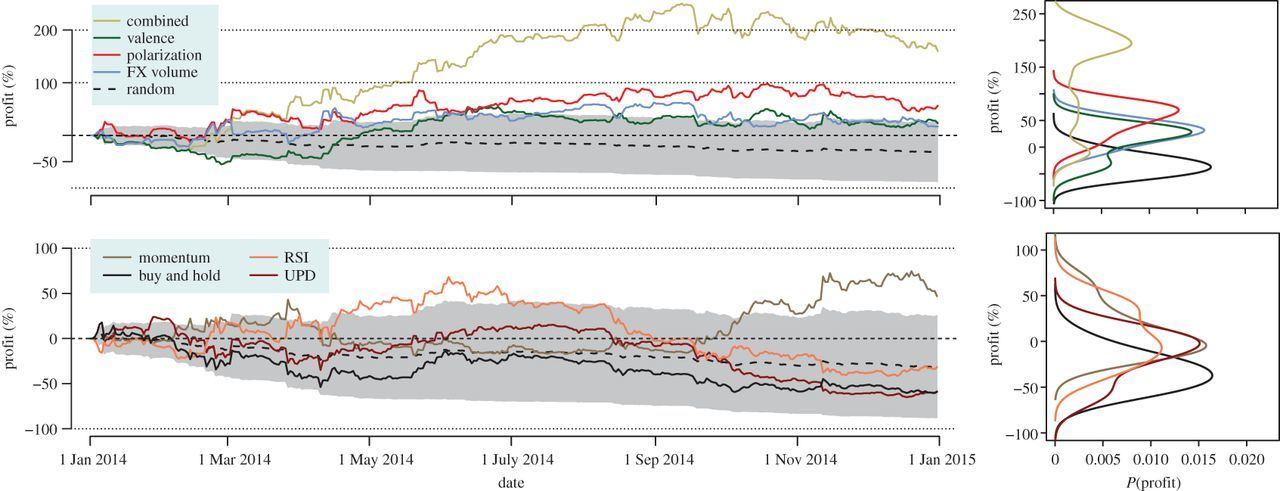
\includegraphics[scale=1.2]{figures/garcia_schweitzer_profits.jpg}
\caption {Comparison of actual profits generated by trading with several different automated investment strategies by \citet{garcia2015}. Polarity and Valence based strategies outperform many traditional strategies.}
\label{fig:garciaschweitzer}
\end{figure*}

\citet{matta2015bitcoin} employ the method of cross-correlation with time-lags of four days in order to explore the correlation between Bitcoin price, the number of positive Tweets, raw Tweet volume and the number of Google searches for Bitcoin. They find a significant cross-correlation for Google Trends and the number of Tweets and Bitcoin price.
\citet{btccovid19} later also explore the correlation between Tweets about Bitcoin and Twitter Sentiment classified with VADER (\citet{vader}) during initial months of the COVID-19 pandemic. They factor in different methods of Tweet preprocessing and different time-lags and  find, that splitting sentences, removing Twitter-specific tags and the combination of these methods lead to an improved correlation of sentiment scores over shorter time-spans. In total however, they find a higher price-correlation of the mere volume of Tweets about Bitcoin than for the actual sentiments. \\
In his Master Thesis, \citet{btcpredictmaster21} takes a different approach by not only analysing the correlation of price and (Twitter) sentiment but trying to actually predict the price of Bitcoin using an LSTM model and feeding in additional sentiment and stance-detection information from algorithmically-selected relevant Crypto-Influencers (as opposed to the whole of Twitter). Lamenting the lack of available Crypto-specific Twitter datasets to train models for the latter tasks on, the author uses fine-tuning methods on a small labelled dataset to introduce Crypto-specific language to the ULMFIT and BERT models he uses. \\
A similar approach, albeit on Chinese data from Sina-Weibo was conducted by \citet{lstmsinaweibo2021} who also use an LSTM for price prediction and a custom Crypto-related dictionary, hand-selected by "crypto domain experts", with information about sentiment (positive, negative, neutral), which they train a RNN from. The authors do not provide too detailed information concerning their methods, but they report a substantial increase in Precision and Recall for Sentiment Analysis on Crypto data compared to an Auto-regressive baseline. \\
Sentiment and a  "bullishness ratio" of aggregated Tweets is used by \citet{KRAAIJEVELD2020101188} to find correlation with prices of various Cryptocurrencies, aided by Granger-Causality-Tests, which imply an effect of sentiment on some Currencies, Tweet volume on some and "bullishness" on others. Generally however, a much larger effect of price increase on Tweet volume and sentiment is found than the other way around. They also discuss the prevalence of Bot Tweets and their methods of identifying them, which I will also dicuss in more detail later. \\
Another more recent example on Bitcoin price prediction through Tweet volume and sentiment comes from \citet{serafini2020}. They compare a volume based model (ARIMAX, an auto-regressive model based on the Moving Average) and a Recurrent Neural Network (LSTM) and find predictive qualities of Twitter Sentiment and a superior performance with the statistical ARIMAX model. \\
I have mentioned Twitter and social media as a vehicle for sentiment transmission, among other things, but to understand the shortcomings of previous analyses of Sentiment Analysis, it is important to take a closer look at language which is employed in the Crypto-space, as it is uniquely idiosyncratic. For one, this is due to the nature of the matters discussed, which are on one hand fairly broad in scope as they extend across Blockchain technology, trading and finance jargon, NFTs, Gaming, etc. On the other hand the idiosyncrasy stems from deliberate use of memetically derived language. Whether the latter serves as a shibboleth which renders the whole scene esoteric to non-initiates is a question to be determined elsewhere but it naturally leads to very poor performances of conventional Sentiment Analysis which are not equipped to derive sentiment valency from words or sentences which are only used, or only have a particular meaning in this context. \\
Table \ref{table:example-tweets} shows a few examples of cryptic language and its actual meaning and sentiment. There are cases where words are re-appropriated, such as "pump", "moon", or "to ape" and cases of neologisms, such as "rekt" (coming from "wrecked"). Many times, acronyms from other sources are borrowed or re-interpreted, such as FUD ("fear, uncertainty, doubt", which describes targeted misinformation campaigns used by the marketing field).

\begin{table}
\renewcommand{\arraystretch}{1.2}
\centering
\caption{\label{table:example-tweets} Some examples of idiosyncratic language used on Crypto-Twitter.}
\begin{tabular}{lll}
\textbf{Tweet Excerpts} & \textbf{Rough Paraphase} & \textbf{Sentiment}  \\ \midrule
"Pump to the moon \emoji{rocket}" & Strong price appreciation. & Positive   \\  
"Don't chase FOMO pumps  & Buying high leads to loss. & Negative\\
or you will get rekt" & & \\
"No more FUD" & No spreading of neg. sentiment. & Positive\\
"LFGGGGG \emoji{rocket}\emoji{rocket}\emoji{rocket}\emoji{rocket}" & Extreme price appreciation. & Positive \\
"Just aped in." & Invested based on emotion. & Neutr./Positive \\
"RELAX HODL \#BabyDoge" & Longer term investment. & Positive \\
\bottomrule
\end{tabular}
\end{table}

A similar problem has been noticed by \citet{loughran} in financial texts, where conventional dictionaries presented a strong negative bias towards three quarters of financial terms, regardless of their positive or neutral meaning in the context. This is the case, for example, due to homonyms. As a reaction to this fact, they have then created  the Loughran McDonald Master Dictionary\footnote{https://sraf.nd.edu/loughranmcdonald-master-dictionary/} incorporating such specific or context-ambiguous terms based on a non-trivial frequency of occurrence in texts and sorting them into one seven sentiment categories. \\
In this project it will be proceeded in a similar way by using the dictionary based Sentiment Classifier VADER, which classifies texts, usually in the format of Tweets, according to a rule-based system. In a similar manner to the problems described above two paragraphs above, its performance on Crypto-specific texts is not very strong. The author therefore plans to adjust its dictionary and associated sentiment scores, relying as much as possible on quantitative methods using frequency analysis, and as little as possible on hand-picking or manual editing. \\
Following this, there will be an attempt at examining the aforementioned assumption of a correlation of Social media sentiment with markets by exploring the relationship of sentiments expressed on Twitter.com concerning certain Crypto projects and their corresponding price movements by looking at their correlation. This is going to be operationalized as a prediction task, like in much of the research mentioned here. However, the nature of the relationship and whether a causality can somehow be inferred is more closely analyzed by introducing a time-lag into a analysis of correlation, similarly to the method \citet{matta2015bitcoin} have employed. This is to see whether change of sentiment precedes price-action or the other way around. \\

\section{Data \& Methods}
\subsection{Data}
The Data used for this project consists of the market data and Tweets which contain the "cashtag" (referring to the token ticker symbol) of four Cryptocurrencies for the time-frame of the whole year of 2021. \\
I should be briefly outlined what influenced the choices of which Cryptocurrencies were chosen for this research. The choices were Cosmos (ATOM), Avalanche (AVAX), Fantom (FTM) and Solana (SOL). They are all Currencies which are used to power their respective Blockchains or nets of Blockchains (as opposed to Tokens, which are Smart Contracts which are deployed on Blockchains), meaning they are roughly comparable in their function. At the same time all of them have been in a medium-size range concerning their market capitalisation, leading an amount of Tweets in the chosen timeframe that is large enough to lend itself to meaningful analysis but still manageable, unlike the amount that talk about high market capitalization Cryptocurrencies like Bitcoin or Ethereum. Generally there is a high amount of price volatility in the Crypto market, but to avoid too erratic price movement I chose not to utilize projects that are too unknown.
\subsubsection{Twitter}
The Twitter data was obtained on the 09.01.2022 using the Twitter Academic Tier API access\footnote{https://developer.twitter.com/en/products/twitter-api/academic-research} which lets users access historical Tweets with a Tweet cap of up to 10 million Tweets per month. The library "Tweepy"\footnote{https://www.tweepy.org/} was used for their convenient methods that function as wrappers around the mere API, such as pagination. The API query was set to the specific cashtag (e.g. \textit{"\$ATOM"}) beginning from 01.01.2021 00:00:00 and ending on 31.12.2021 23:59:59 and the English language. To gather a set of baseline Tweets, which do not concern themselves with Cryptocurrencies (from now on referenced as "Vanilla"), the query was set empty and collected all Tweets during four separate timeframes in 2021 of five minutes each, which amounted to a roughly equal sized dataset as each of the Crypto datasets. Besides the Tweet text, the information obtained through the API also contains account name, number of followers, number of author's tweets, author description, author location, timestamp, number of likes, number of re-tweets, number of comments and quote count. \\

\begin{table}
\renewcommand{\arraystretch}{1.2}
\centering
\caption{\label{table:tweet-counts} Number of raw Tweets obtained from the API.}
\begin{tabular}{ll}
\textbf{Dataset} & \textbf{Number of Tweets}  \\ \midrule
Cosmos (ATOM) & 359,955   \\  
Avalanche (AVAX) & 651,672 \\
Fantom (FTM) &  502,361 \\
Solana (SOL) &  2,861,546 \\
Vanilla & 1,000,000 \\
\bottomrule
\end{tabular}
\end{table}

\subsubsection{Market}
The market data was obtained on the 11.01.2022 via the Binance Data Collection\footnote{https://data.binance.vision/}. Binance is the largest Cryptocurrency exchange with 28.5 million users as of 2021\footnote{Source: cryptocompare.com}. The data is in the format of Kline data, also known as Candlesticks, which contain, among other things, the open, close, highest and lowest price and the trading volume for a certain time-interval \ref{fig:candlestick}. The time-intervals obtained were one day, twelve hours, four hours and one hour for each of the Cryptocurrencies mentioned in the paragraph above and for the time-frame of 2021. \\
One thing which should be noted when looking at Figure \ref{fig:coingecko2021}, is that all four exhibit a similar pattern and a bias towards price appreciation during 2021. \\

\begin{figure}
     \centering
     \begin{subfigure}[b]{0.4\textwidth}
         \centering
         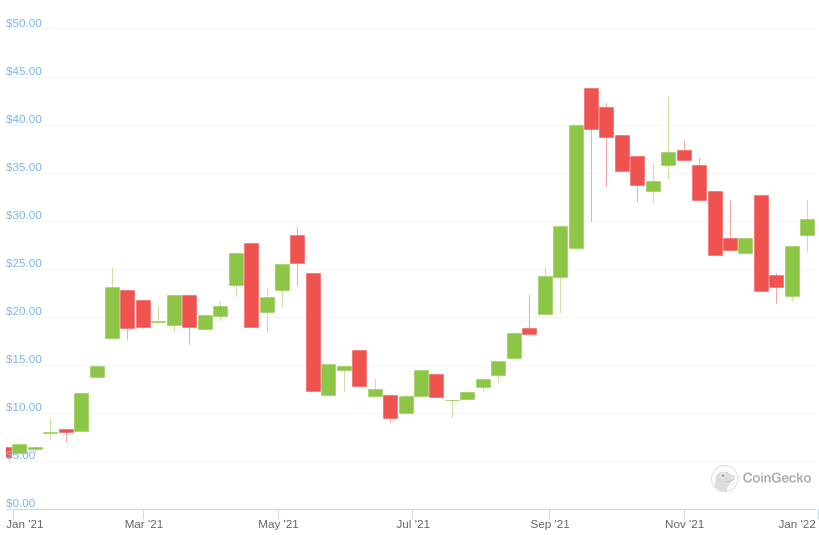
\includegraphics[width=\textwidth]{figures/atom2021.png}
         \caption{ATOM}
         \label{atom2021}
     \end{subfigure}
     \hfill
     \begin{subfigure}[b]{0.4\textwidth}
         \centering
         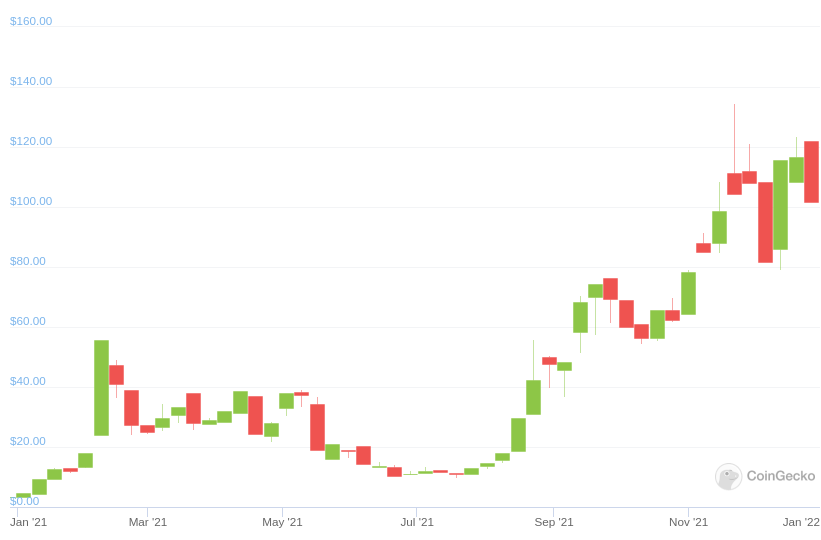
\includegraphics[width=\textwidth]{figures/avax2021.png}
         \caption{AVAX}
         \label{avax2021}
     \end{subfigure} 
     \hfill \\
     \begin{subfigure}[b]{0.4\textwidth}
         \centering
         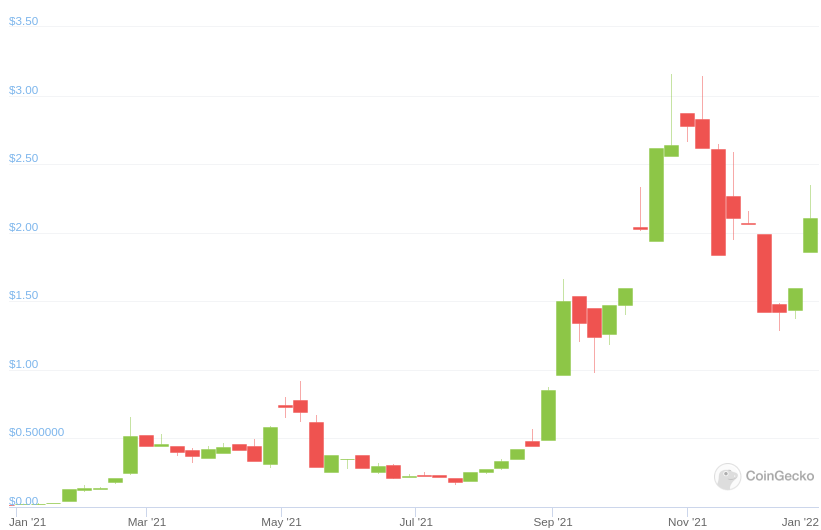
\includegraphics[width=\textwidth]{figures/ftm2021.png}
         \caption{FTM}
         \label{ftm2021}
     \end{subfigure}
      \hfill
     \begin{subfigure}[b]{0.4\textwidth}
         \centering
         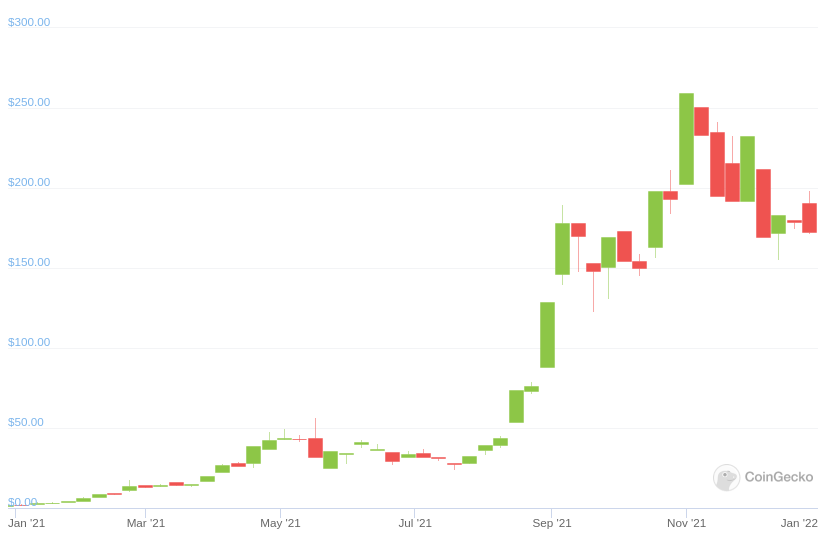
\includegraphics[width=\textwidth]{figures/sol2021.png}
         \caption{SOL}
         \label{sol2021}
     \end{subfigure}
        \caption{Complete 2021 price charts for Cryptocurrencies used in this project. (Source: coingecko.com)}
        \label{fig:coingecko2021}
\end{figure}

\begin{figure*}
\centering
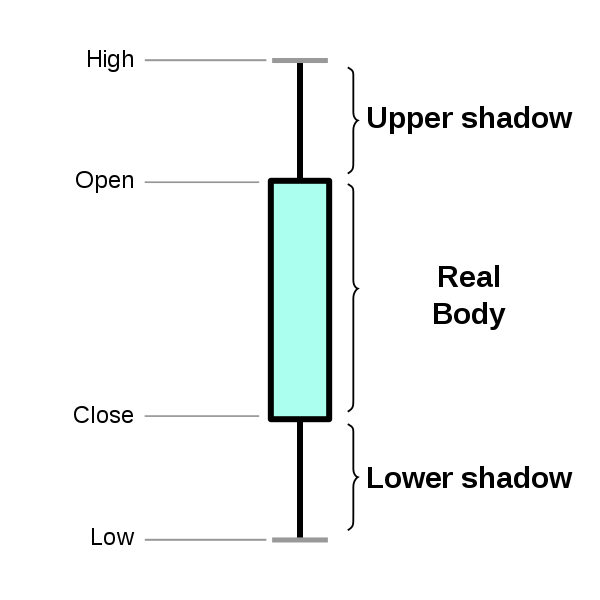
\includegraphics[scale=0.2]{figures/candlestickwiki.png}
\caption {Kline Candlestick. (Source: en.wikipedia.org/wiki/Candlestick\_chart)}
\label{fig:candlestick}
\end{figure*}

\subsubsection{Preprocessing}
After describing some of the qualities of and the process of obtaining the data used in this project, in this section I will describe the various methods of processing employed. In order to analyse the word frequencies of the Crypto-related Tweets, the Tweets are aggregated into corpora, one for Crypto-related Tweets and one that is Vanilla. This is preceded by some pre-processing steps, which are as follows:

\begin{enumerate}
  \item Tweets that contain words identifying them as bot-created content are removed.
  \item Tweets which contain more than 6 amount of any tag (\#, \$, @) are removed. 
  \item Twitter Tags (\#, \textdollar, @) are removed from Tweets. 
  \item Words from the NLTK Stop words Corpus\footnote{https://www.nltk.org/nltk\_data/} are removed.
  \item Lower Case is applied to all words.
  \item Tweets are word-tokenized.
\end{enumerate}
I arrived at the initial list of words which should identify bot-created Tweets through preliminary qualitative exploration of the data and the methods \citet{KRAAIJEVELD2020101188} describe. I have found that spamming Twitter tags are also a good indicator for inorganic content.

\begin{figure*}
\centering
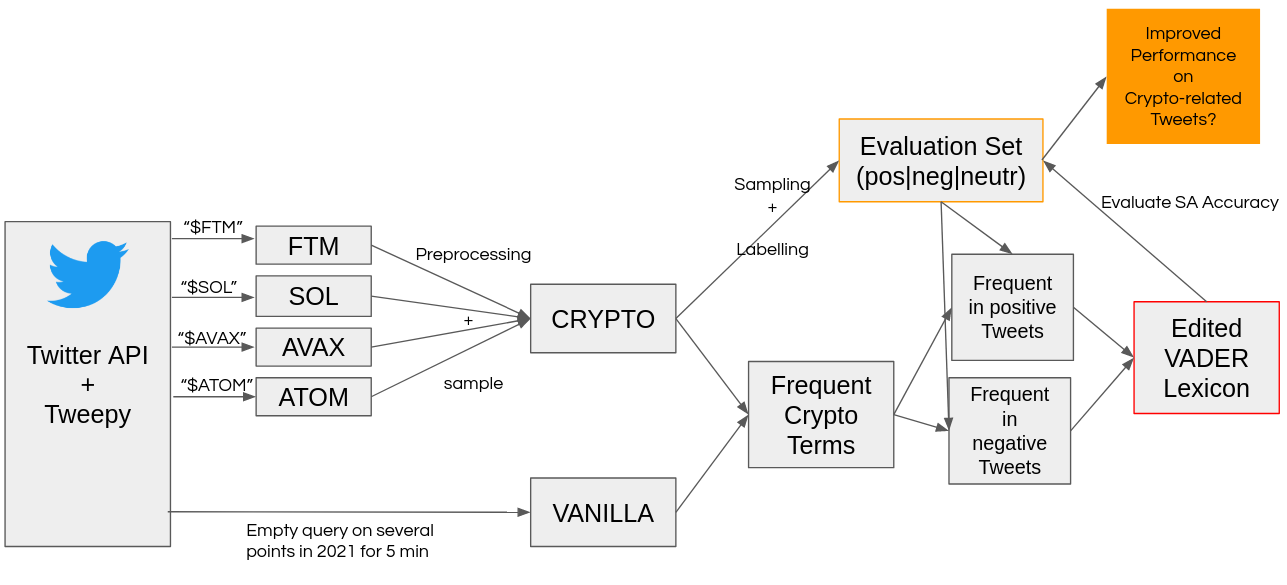
\includegraphics[scale=0.5]{figures/twitter_pipeline.png}
\caption {Pre-processing Pipeline for Twitter Data}
\label{fig:twitter_pipeline}
\end{figure*}

\subsection{Gold standard creation}
A gold-standard subset of the Twitter data is needed as a basis for the creation of the VADER dictionary edits and for the final evaluation of the classifiers. As of writing, for Crypto-related Twitter data, such a dataset does not exist and will therefore be created in the scope of this project by manual labelling until a size of n = 3000 Tweets is reached. \\
Initially the subset is sampled randomly from the Crypto-Tweet dataset, in order to eliminate any bias concerning temporal up or down-trends and to have roughly even parts of Tweets about all four chosen Cryptocurrencies. \\
The labelling is done into "positive", "negative" and "neutral" categories and according to the authors own knowledge of the language employed in the Crypto space. The data is then split 4:1 into a subset with which to edit VADER's dictionary and a subset to evaluate the performance on, in order to not contaminate the evaluation process with examples already "seen" by the classifier. \\

\subsection{Frequency Analysis}
In order to determine which words are the relevant words in the Cryptocurrency context, the Difference (see: Set Theory) is computed of the top 500 most frequently occurring words of the Crypto-related and Vanilla Corpora. \\
In a second step, the positive and negative valency of this set of words is determined by analysing the relative frequencies in which they occur in the positive, respective negative Tweets in the labelled Gold standard subset. This is again visually represented in Figure \ref{fig:frequent_terms}. \\

\begin{figure*}
\centering
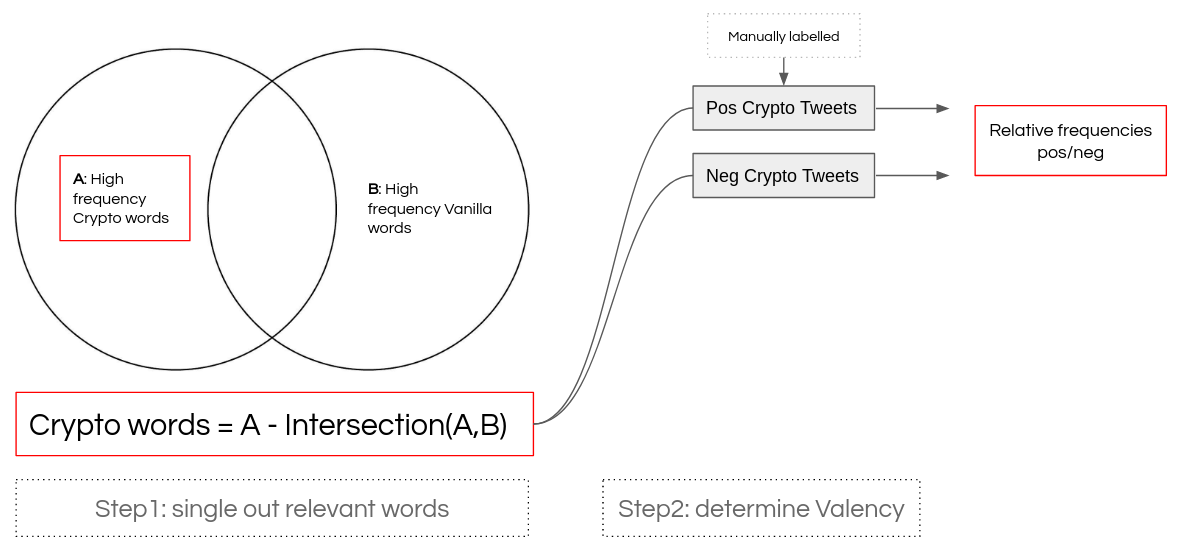
\includegraphics[scale=0.55]{figures/frequent_terms.png}
\caption {Determining frequent Twitter specific terms.}
\label{fig:frequent_terms}
\end{figure*}


\subsection{Dictionary Edit}
In order to improve performance of the Sentiment Analysis Classifier on Crypto-related Tweets, once the relative frequencies of positive and negative Tweets are determined, the next step is to edit the VADER's dictionary in a way that will reflect the increased occurrence of these words and their valency concerning sentiment. A short overview of how VADER works to begin with:

\subsubsection{VADER Sentiment Analysis Classifier} 
VADER is a rule-based model for general Sentiment Analysis developed by \citet{vader}. Its core piece is a dictionary of words, which are paired with human-generated sentiment scores in a range of -4 (extremely negative) and 4 (extremely positive). The final scores are the mean of the scores of ten human ratings. In addition to the dictionary of sentiment-laden words, there is a lists of words which indicate negation or amplification, along with a small set of phrases, which are used in the rule-based generation of the sentiment scores. The output of the classifier consists of separate scores for positive, negative and neutral sentiment, as well as a compound score calculated from the latter three.

\subsubsection{Crypto-edited VADER}
The way editing of the VADER dictionary was approached in this project was to infer the sentiment of words by the frequency of their occurrence in positive, respective negative Tweets. To do this, the relative frequencies of occurrence of Crypto-specific words in positive/negative Tweets were taken and normalized within the range of possible VADER scores and then appended to VADER's dictionary if there was no entry and replaced if there was one. Looking at the distribution, what quickly becomes apparent is a skew towards positive sentiment words, which is an expected result of the imbalance of positive and negative Tweets in total. \\ 

\begin{figure}[H]
\centering
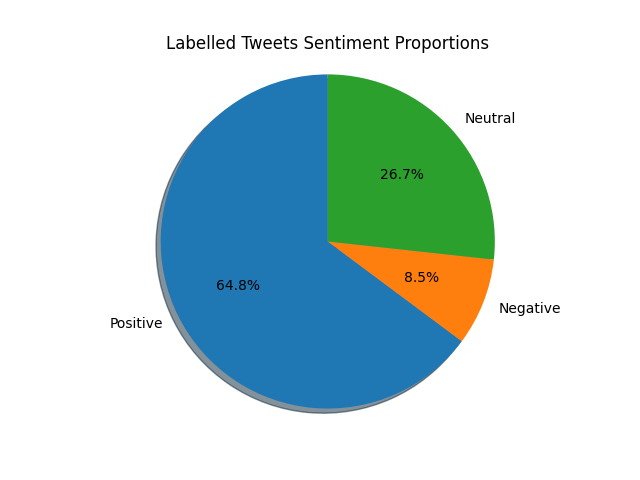
\includegraphics[scale=0.6]{figures/gold_sentiment_proportions.png}
\caption {Shares of positive, negative and neutral Tweets of gold standard labelled Tweet data set}
\label{fig:gold_standard_proportions}
\end{figure}

First, for each of the Crypto-relevant words, a valency count is created based on number of occurrences in positive and negative Tweets, from here on referred to as "PosNeg score". 

\begin{equation}
PosNeg\_score = n\_occurences\_in\_pos\_tweets - n\_occurences\_in\_neg\_tweets
\end{equation}

Then, VADER scores are assigned according to assignment table below. Due to the much lower number of words with negative sentiment and resulting low PosNeg scores, positive and negative sides of the scale have to be handled very differently \\

\begin{table}[H]
\renewcommand{\arraystretch}{1.2}
\centering
\caption{\label{table:vader-score-assignment} VADER score assignments from PosNeg score.}
\begin{tabular}{ll}
\textbf{PosNeg score range} & \textbf{VADER score} \\ \midrule
(50,  max) & 4   \\  
(20,  49) & 3   \\ 
(10,  19) & 2   \\ 
(-1,  9) & discard   \\ 
(-2, -4) & -2   \\ 
(-5, -9) & -3   \\ 
(-10, min) & -4   \\ 
\bottomrule
\end{tabular}
\end{table}

Most words' scores are concentrated around the middle of the scale. Overwriting all the existing scores in the dictionary with the derived scores would therefore lead to a possible neutralization of many terms which may before have carried stronger sentiment, which was useful to the Sentiment Analysis task. To avoid this, a number of words with lower absolute values were discarded according to a set range in the rule-based VADER score assignment method. \\

\begin{figure}[H]
     \centering
     \begin{subfigure}[b]{0.45\textwidth}
         \centering
         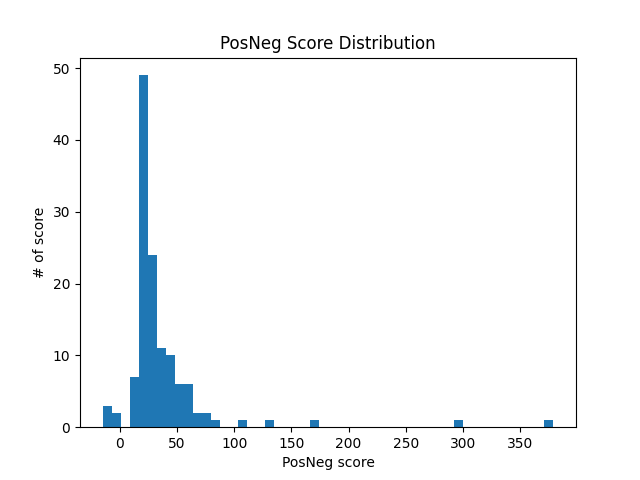
\includegraphics[width=\textwidth]{figures/posneg_words_posneg_score.png}
         \caption{Distribution of Pos/Neg scores of Crypto-relevant words}
         \label{posneg_dist}
     \end{subfigure}
     \hfill 
     \begin{subfigure}[b]{0.45\textwidth}
         \centering
         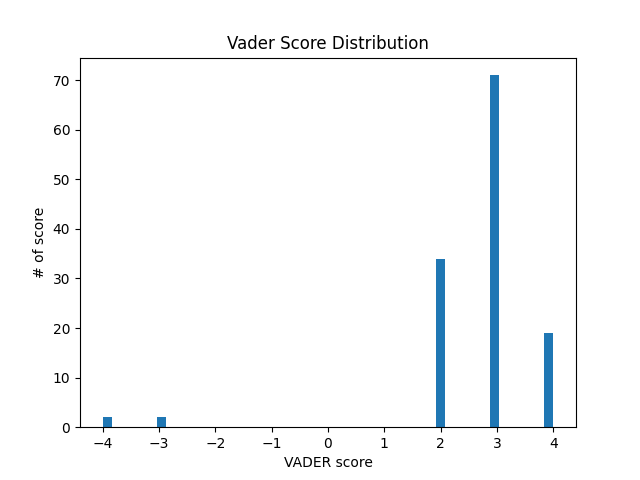
\includegraphics[width=\textwidth]{figures/posneg_words_vader.png}
         \caption{Distribution of VADER scores of Crypto-relevant words according to rule-based assignment.}
         \label{vader_dist}
     \end{subfigure}
\end{figure}

\subsection{Time-lagged Correlation}
The Cross-Correlation is a statistical method, which measures the temporal similarity between two time series. In this example, the method of Cross-Correlation implemented was the Pearson product-moment correlation coefficient. different positive and negative Time-lags are introduced to infer the causal temporal relationship. In essence, what this does is to shift one of the sequences by a defined lag and calculate the correlation. \\


\begin{equation}
r = \frac{n(\Sigma xy) - (\Sigma x)(\Sigma y)}{\sqrt{[n\Sigma x^2 - (\Sigma x)²] [n\Sigma y^2 - (\Sigma y)²]}}
\end{equation}
The above equation is the Pearson correlation formula used to determine the time-lagged Cross-correlation, $x_i$ and $y_i$ being the values of the respective sequences. \\

For the final step of analysing the time-lagged correlation, the Twitter and corresponding Market data are aggregated. For several possible time-intervals (1h, 4h), the sentiment scores for all of the Tweets which fall between the Open and the Close timestamp of said time-interval are computed and averaged. Also, the mere number of Tweets in this timestamp are added and recorded as Tweet Volume. The outcome of this is a sequence of Candlesticks which do not only contain information about the price, but about the average sentiment of Twitter and the Tweet Volume in this time-frame. \\

\section{Results}

\subsection{Sentiment Analysis}
The accuracy of sentiment prediction of VADER using the Vanilla lexicon vs. the edited lexicon was compared on the whole gold standard data set and on the holdout test set, which makes up 20\% of the gold standard set, which was not not used to edit VADER's lexicon. Accuracy of the possible predictions "positive", "neutral" and "negative", and the overall accuracy score, are displayed on confusion matrices below on Figure \ref{fig:confusion}.

\newgeometry{right=5mm, left=5mm}

\begin{figure}[H]
     \centering
     \begin{subfigure}[b]{0.45\textwidth}
         \centering
         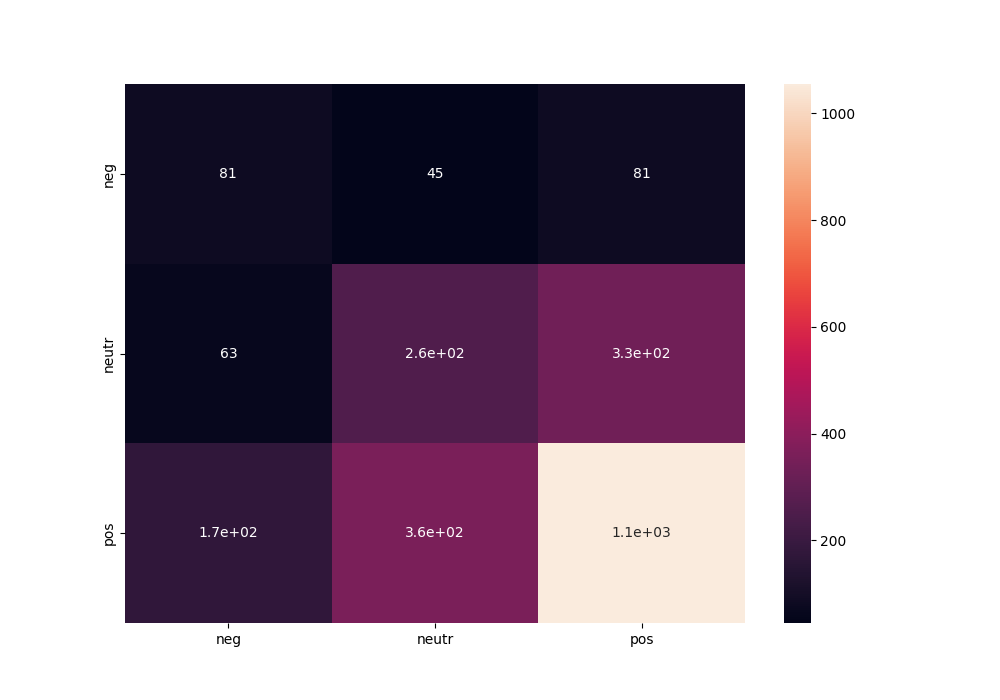
\includegraphics[width=\textwidth]{figures/confusion_matrix_vader_vanilla_acc_0593_full_data.png}
         \caption{Vanilla VADER on whole labelled set (Accuracy: 0.593)}
         \label{matrix_van_full}
     \end{subfigure}
     \hfill
     \begin{subfigure}[b]{0.45\textwidth}
         \centering
         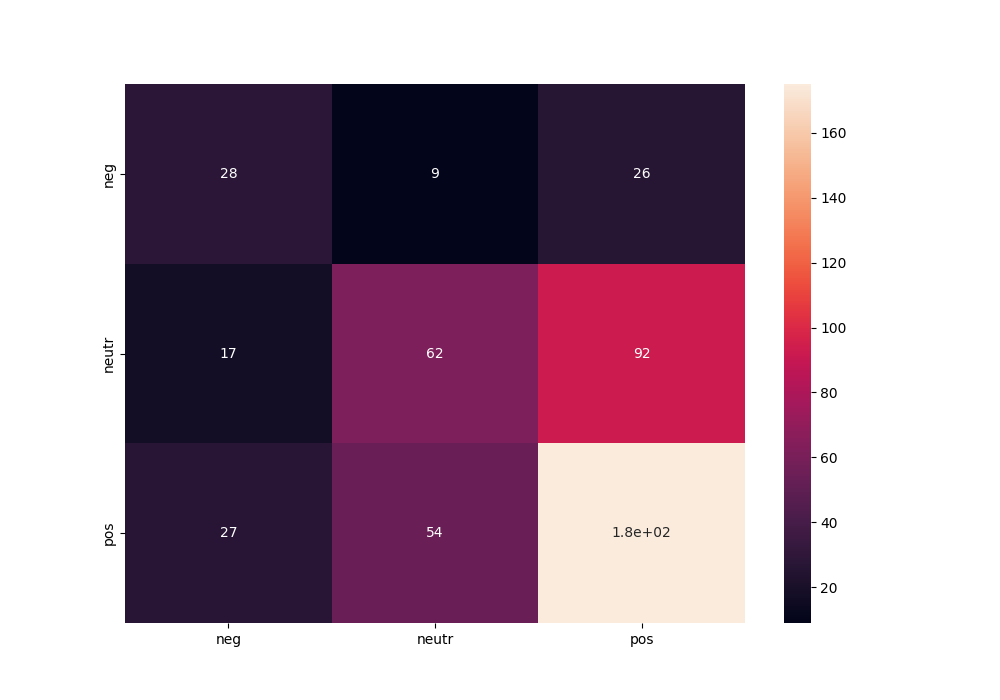
\includegraphics[width=\textwidth]{figures/confusion_matrix_vader_vanilla_testset_0541.png}
         \caption{Vanilla VADER on labelled test set (Accuracy: 0.541)}
         \label{matrix_van_test}
     \end{subfigure} 
     \hfill \\
     \begin{subfigure}[b]{0.45\textwidth}
         \centering
         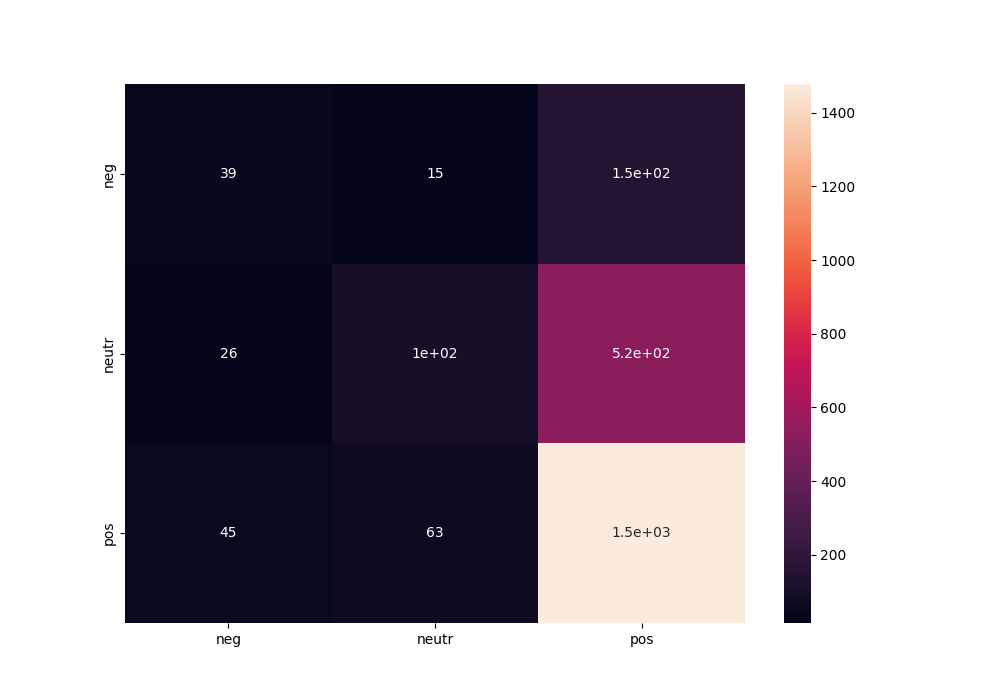
\includegraphics[width=\textwidth]{figures/confusion_matrix_vader_bins_acc_0662_full_data.png}
         \caption{Edited VADER on whole labelled set (Accuracy: 0.662)}
         \label{matrix_van_full}
     \end{subfigure}
      \hfill
     \begin{subfigure}[b]{0.45\textwidth}
         \centering
         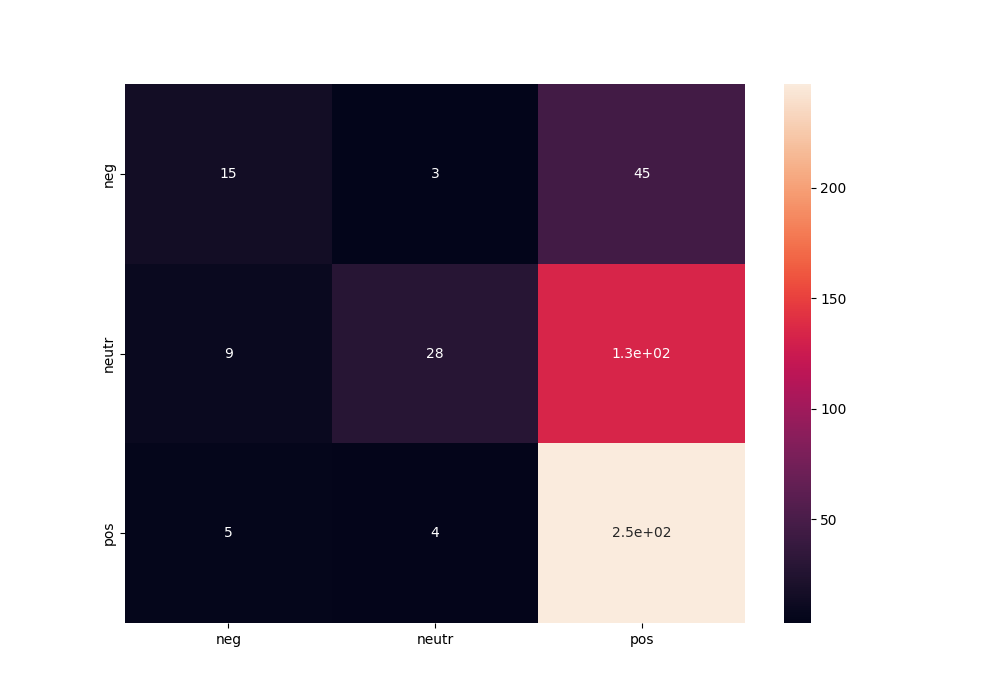
\includegraphics[width=\textwidth]{figures/confusion_matrix_vader_bins_testset_0592.png}
         \caption{Edited VADER on labelled test set (Accuracy: 0.592)}
         \label{matrix_van_test}
     \end{subfigure}
        \caption{Comparison of Confusion matrices and accuracies of Vanilla and Edited VADER classifier applied to whole labelled dataset and on the holdout test set not used for editing the VADER dictionary (train test split: 80/20).}
        \label{fig:confusion}
\end{figure}

\restoregeometry     %so it does not affect the rest of the pages.

\begin{figure}[H]
     \centering
     \begin{subfigure}[b]{0.45\textwidth}
         \centering
         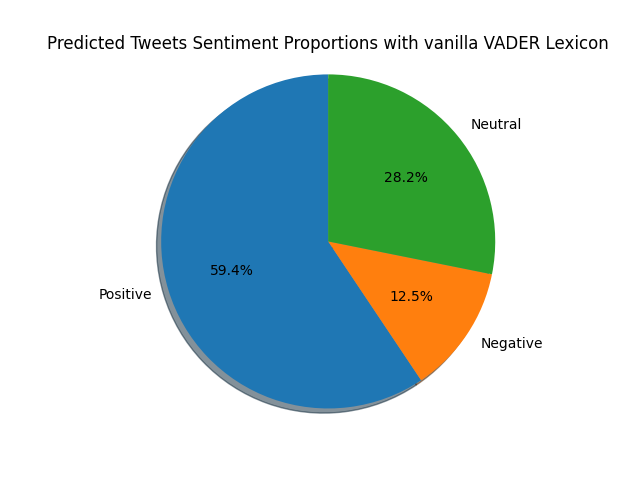
\includegraphics[width=\textwidth]{figures/predicted_sentiment_proportions_vanilla.png}
         \caption{Shares of positive, negative and neutral Tweets of Vanilla VADER predictions}
         \label{vanilla_pie}
     \end{subfigure}
     \hfill 
     \begin{subfigure}[b]{0.45\textwidth}
         \centering
         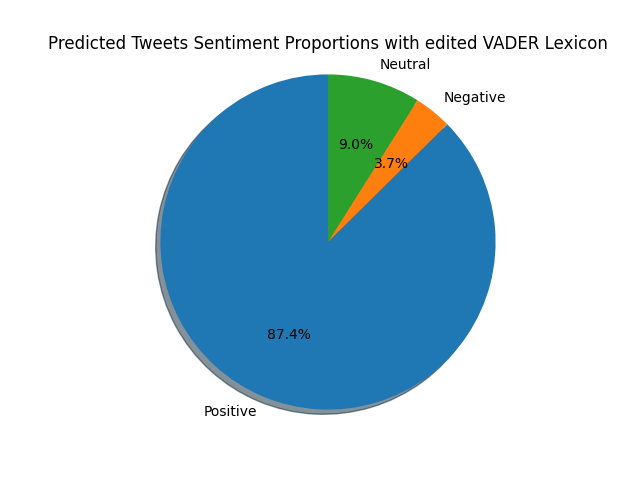
\includegraphics[width=\textwidth]{figures/predicted_sentiment_proportions_edited.png}
         \caption{Shares of positive, negative and neutral Tweets of edited VADER predictions}
         \label{edit_pie}
     \end{subfigure}
        \caption{It becomes clear that the edited classifier has developed a bias towards positive predictions. Vanilla VADER prediction proportions are much closer to the gold standard proportions (See Fig \ref{fig:gold_standard_proportions})}
        \label{fig:vader_piechart_comparison}
\end{figure}

\subsection{Time-lagged Cross-Correlation}

Below, there are several things plotted: Cryptocurrency price, Tweet volume, Mean Twitter sentiment and the Time-Lagged Cross-Correlation. One can imagine the time-lag as shifting the Price Change sequence along the respective other sequence and calculating the correlation as if the Price Change had preceded or anteceded the respective other sequence. This is to see if there is an implication of causality. This is done for all of the Cryptocurrencies, and for different time-lag steps and candlestick intervals. A Time-lag of 0 implies simultaneity.\\

\newgeometry{right=5mm, left=5mm}

\begin{figure}[H]
     \centering
     \begin{subfigure}[b]{0.45\textwidth}
         \centering
         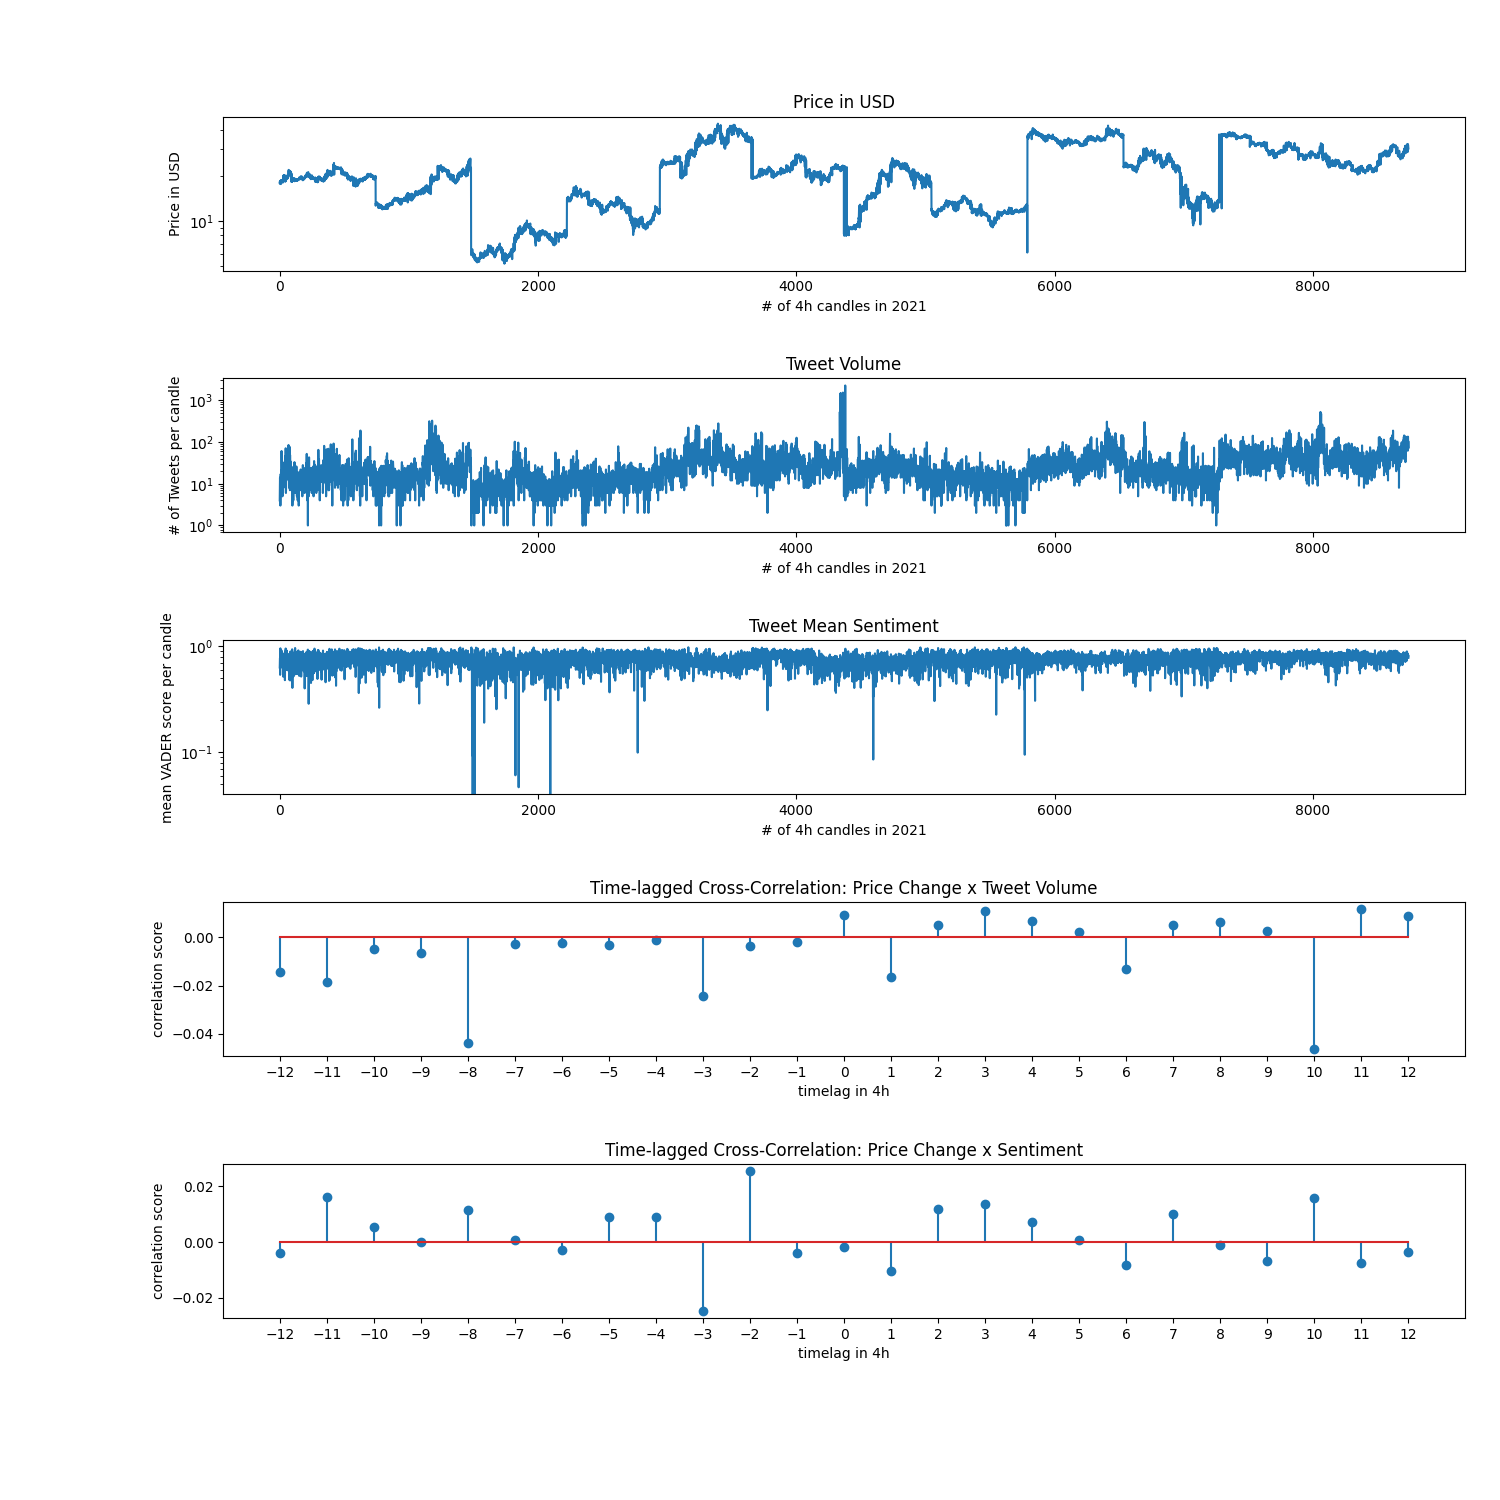
\includegraphics[width=\textwidth]{figures/crosscorrATOM_1h_range(-12, 13).png}
         \caption{ATOM 1H}
         \label{atom1h}
     \end{subfigure}
     \hfill 
     \begin{subfigure}[b]{0.45\textwidth}
         \centering
         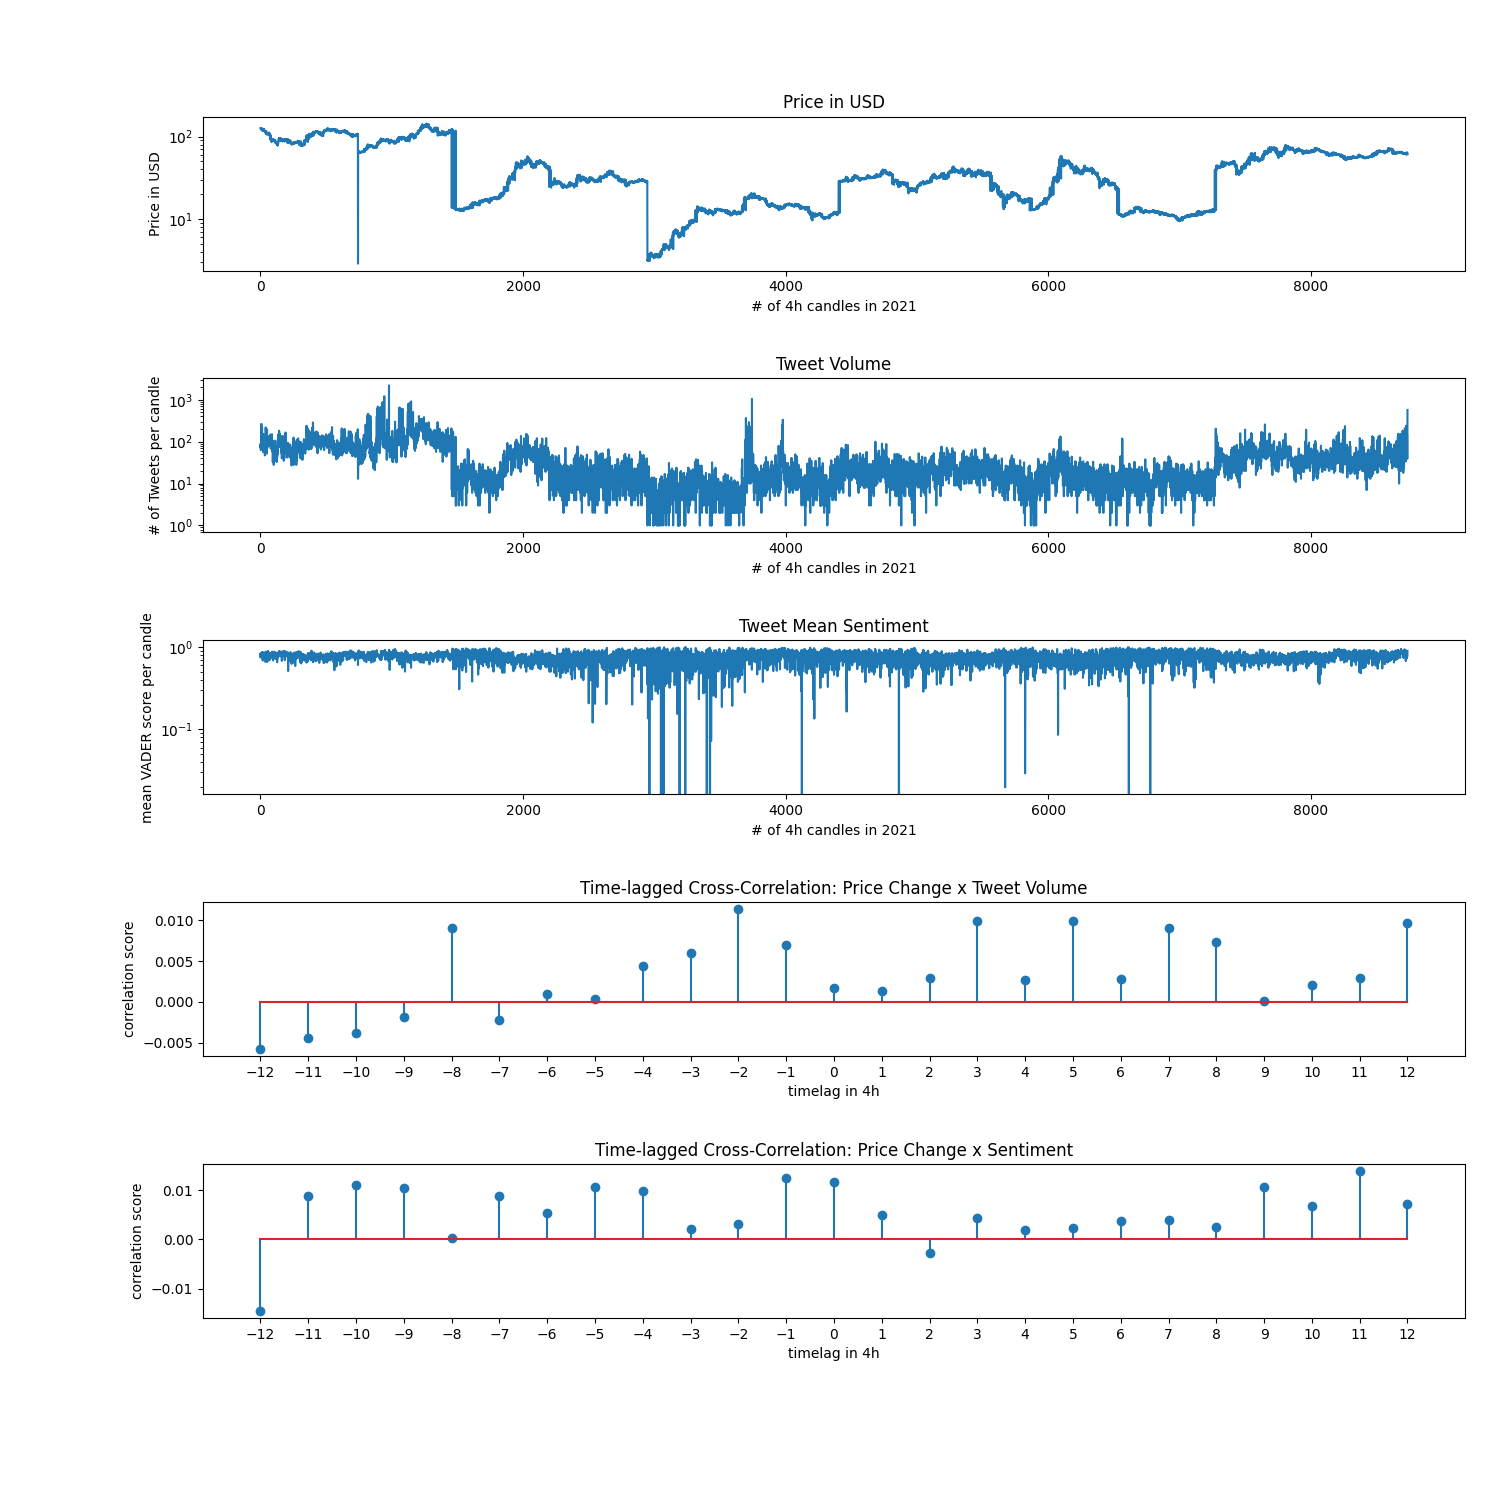
\includegraphics[width=\textwidth]{figures/crosscorrAVAX_1h_range(-12, 13).png}
         \caption{AVAX 1H}
         \label{AVAX 1H}
     \end{subfigure} 
     \hfill \\
     \begin{subfigure}[b]{0.45\textwidth}
         \centering
         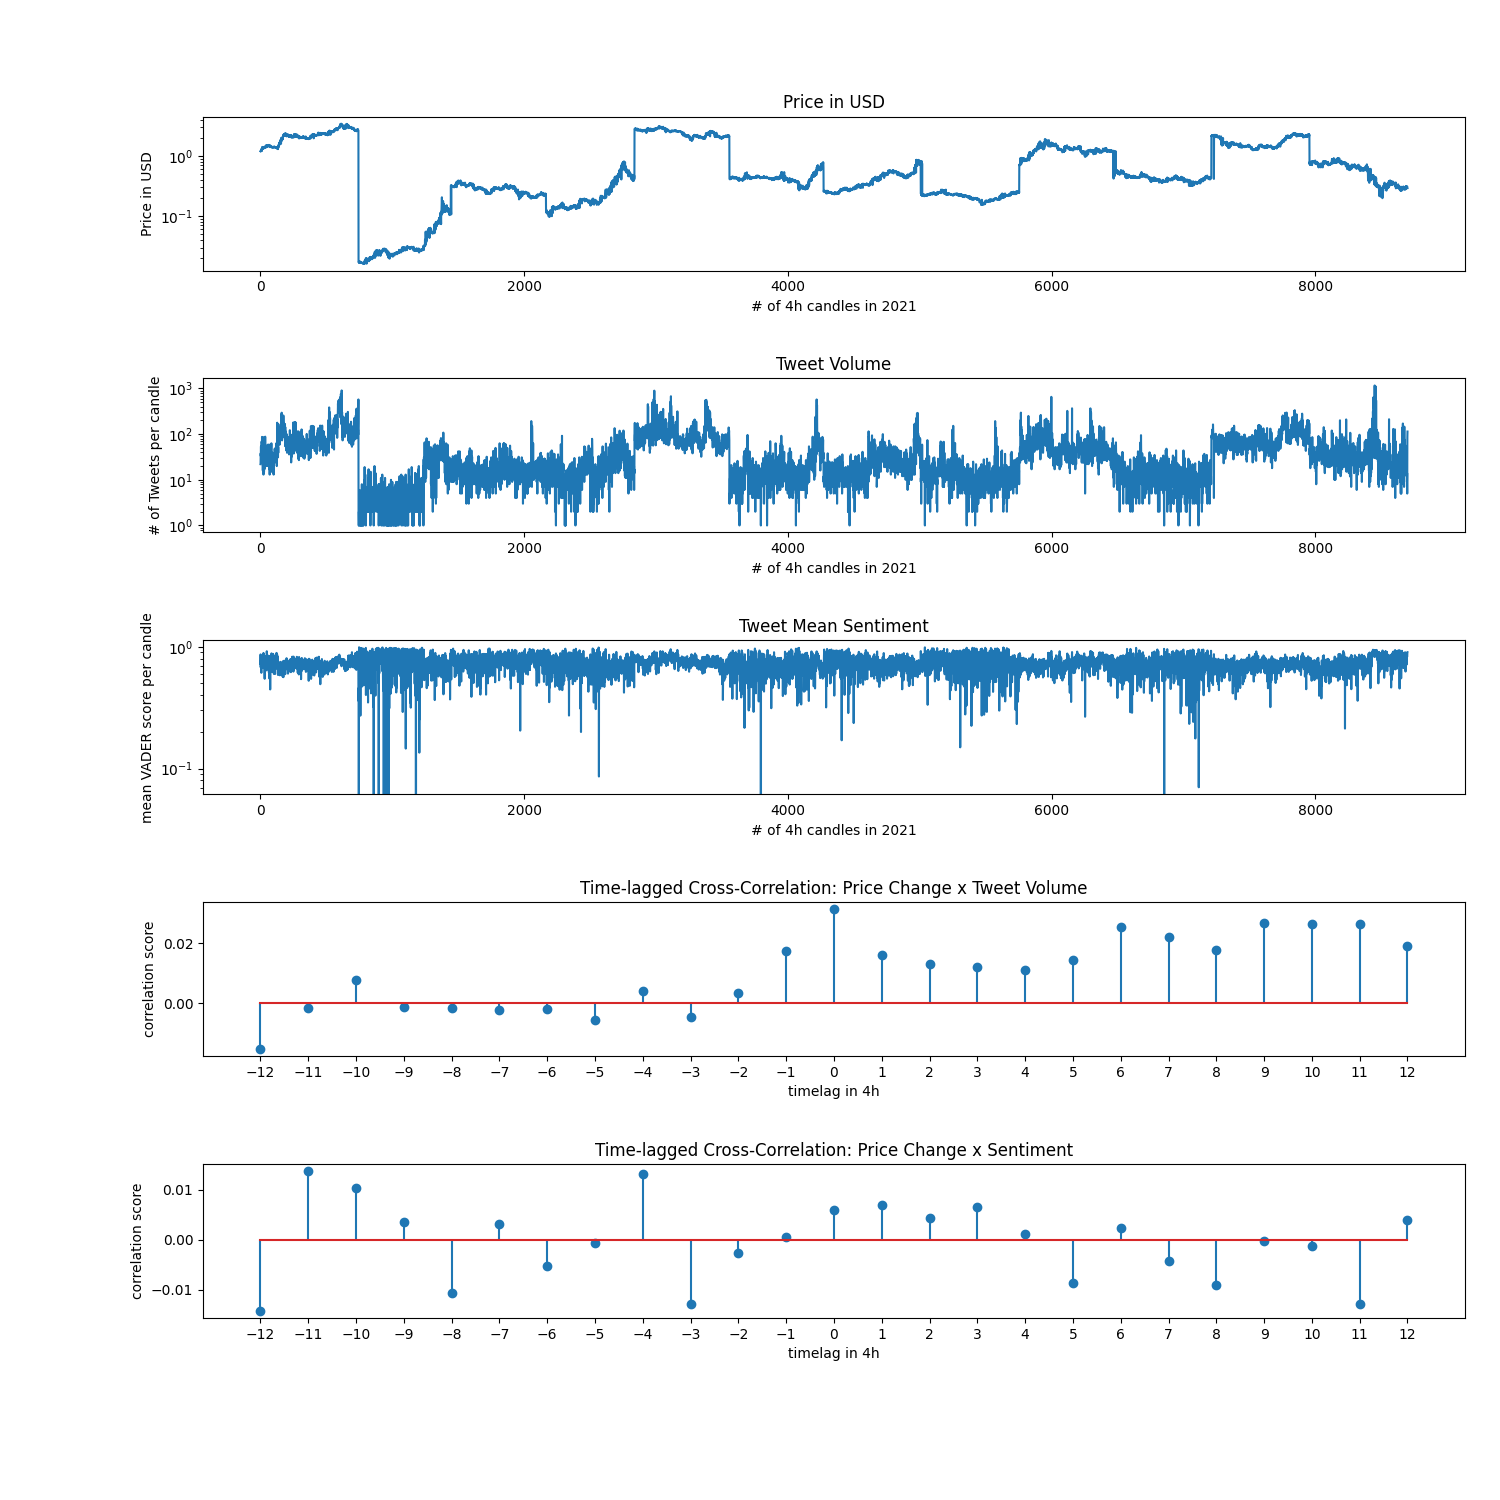
\includegraphics[width=\textwidth]{figures/crosscorrFTM_1h_range(-12, 13).png}
         \caption{FTM 1H}
         \label{ftm1h}
     \end{subfigure}
      \hfill 
     \begin{subfigure}[b]{0.45\textwidth}
         \centering
         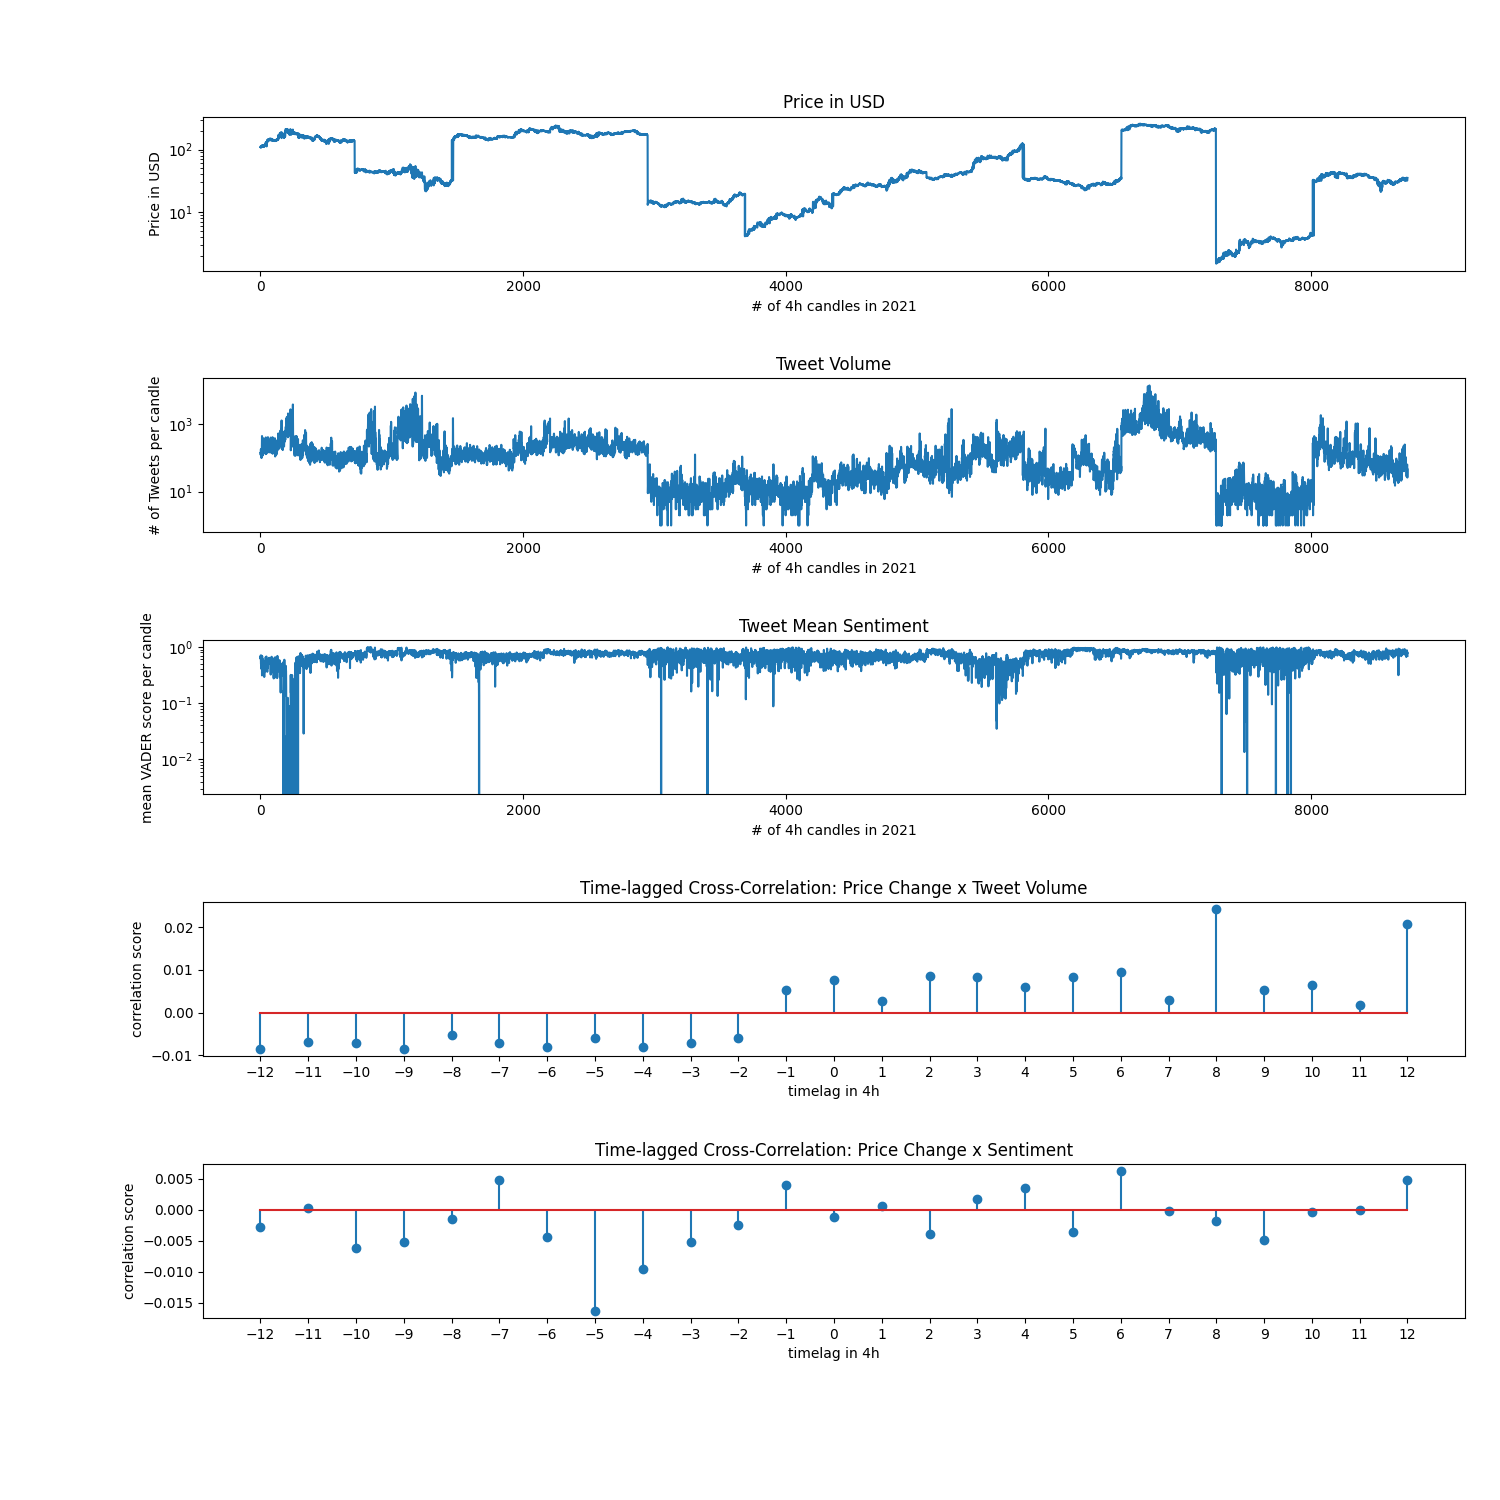
\includegraphics[width=\textwidth]{figures/crosscorrSOL_1h_range(-12, 13).png}
         \caption{SOL 1H}
         \label{sol1h}
     \end{subfigure}
        \caption{Price, Tweet Volume, Tweet Sentiment and Cross-Correlation graphs of Tweet Volume x Price and Tweet Sentiment x Price. This is using the 1h candles for the four chosen Cryptocurrencies.}
        \label{fig:crosscorr-1h}
\end{figure}

\begin{figure}[H]
     \centering
     \begin{subfigure}[b]{0.45\textwidth}
         \centering
         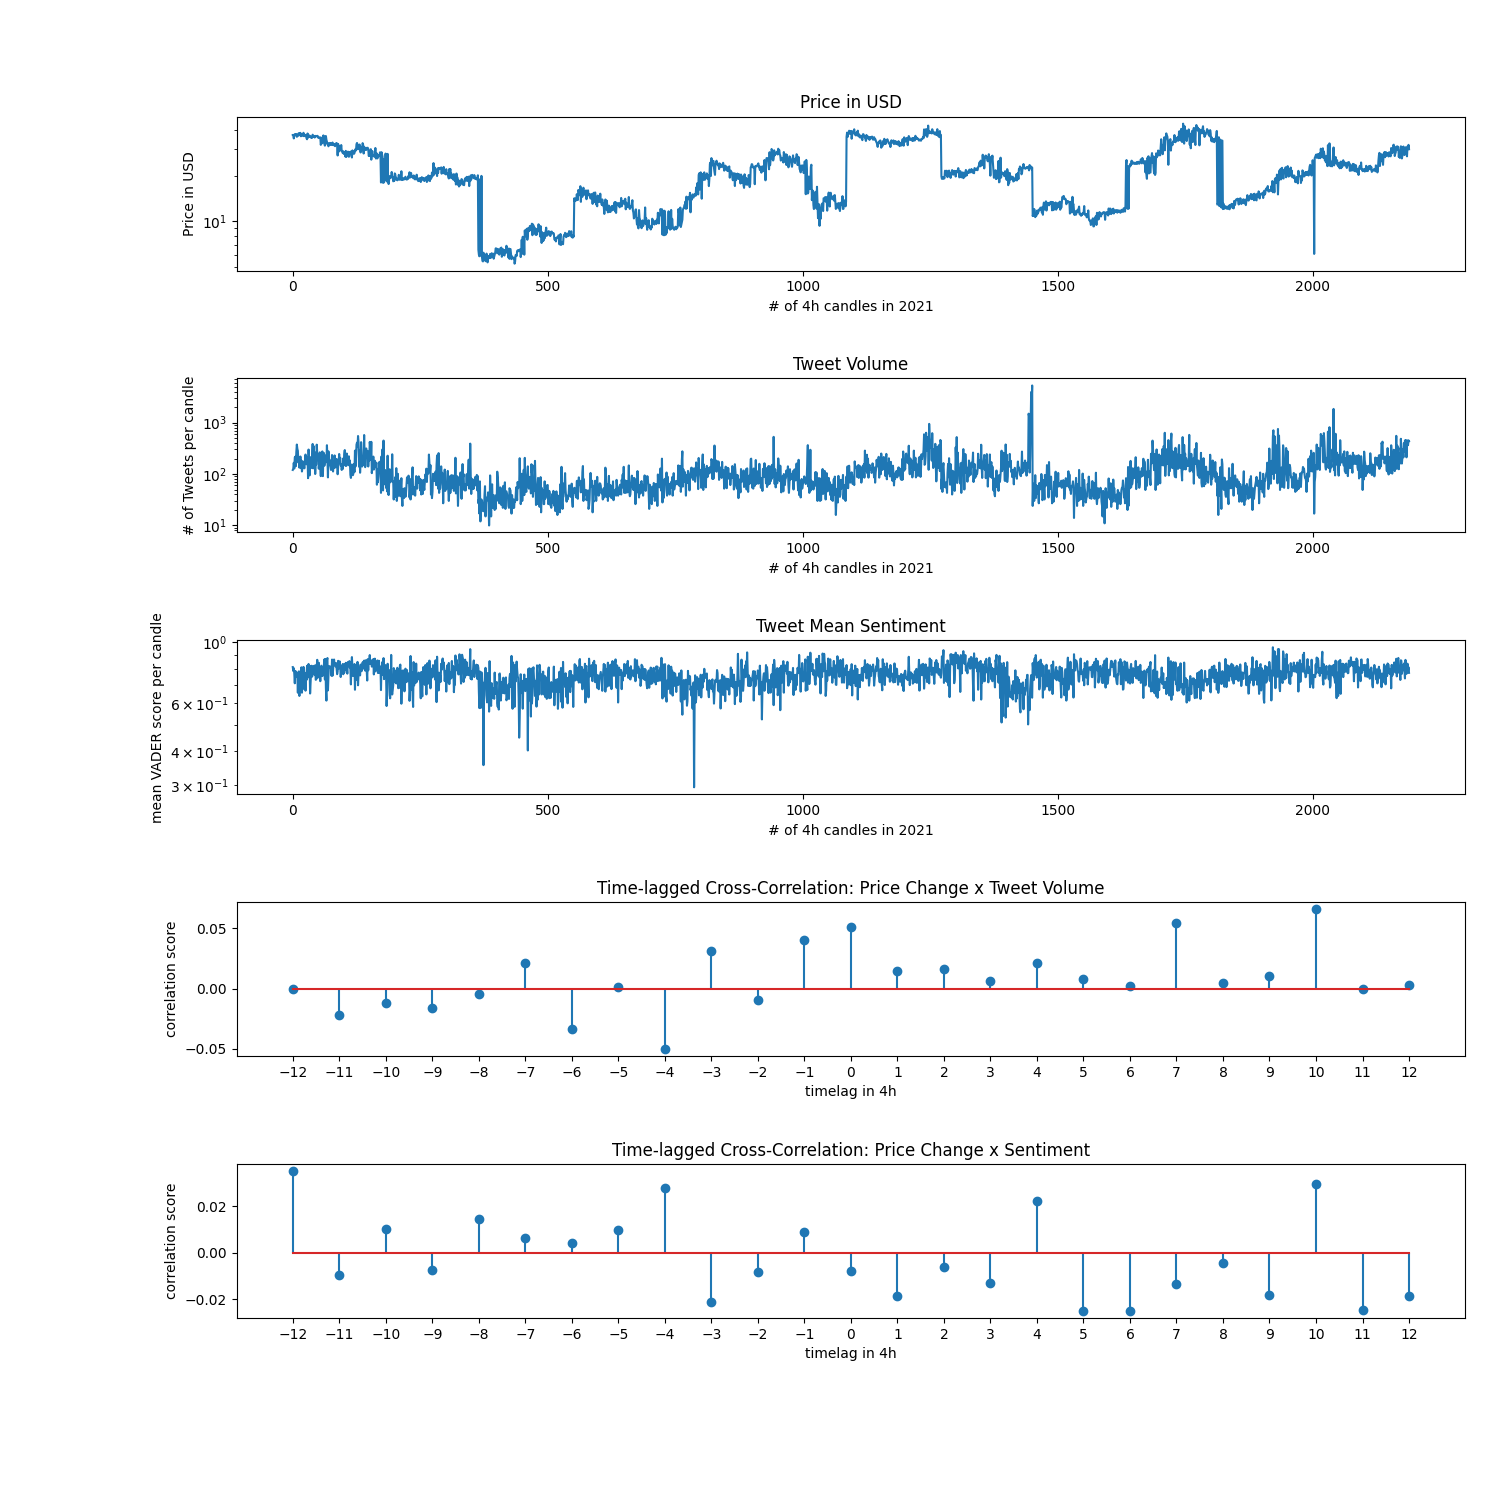
\includegraphics[width=\textwidth]{figures/crosscorrATOM_4h_range(-12, 13).png}
         \caption{ATOM 4H}
         \label{atom4h}
     \end{subfigure}
     \hfill 
     \begin{subfigure}[b]{0.45\textwidth}
         \centering
         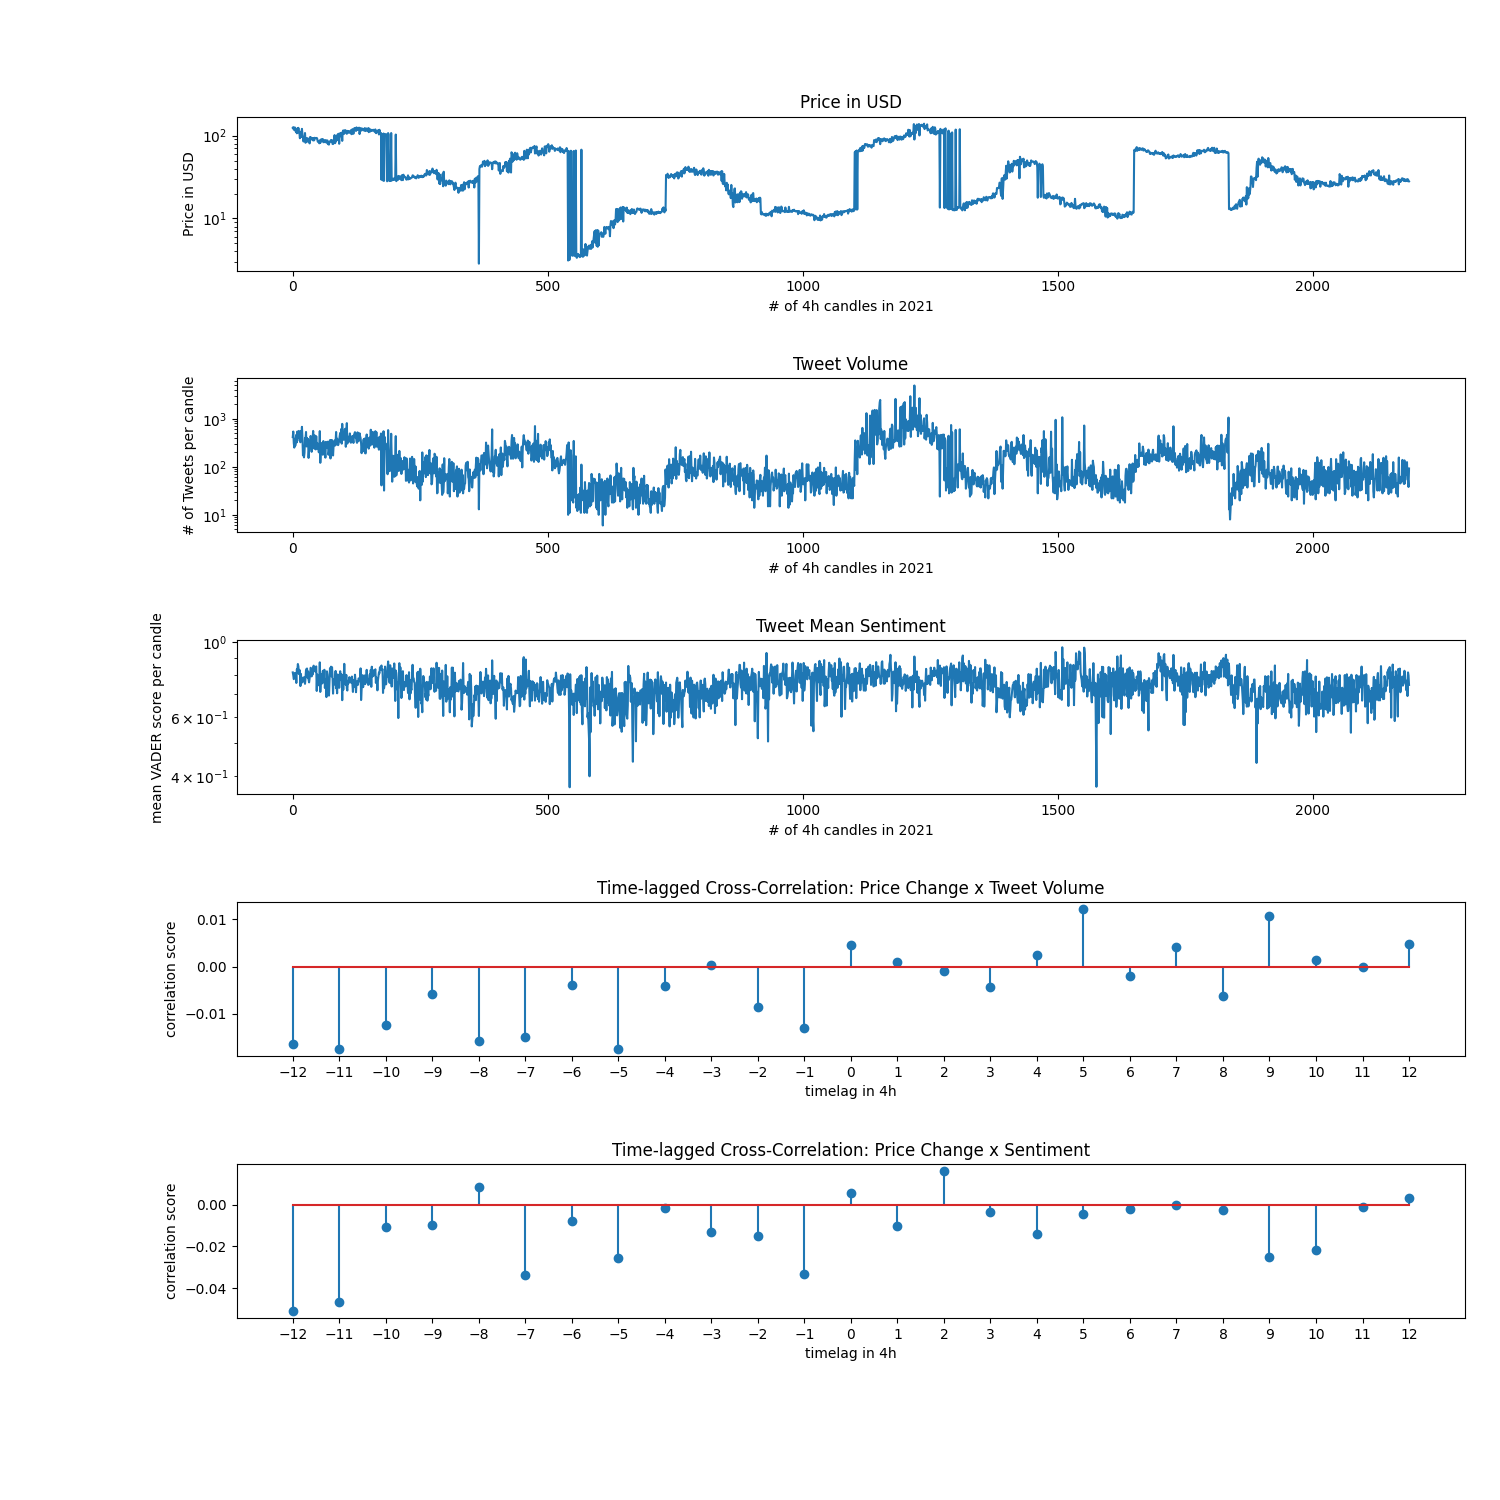
\includegraphics[width=\textwidth]{figures/crosscorrAVAX_4h_range(-12, 13).png}
         \caption{AVAX 4H}
         \label{AVAX 4H}
     \end{subfigure} 
     \hfill \\
     \begin{subfigure}[b]{0.45\textwidth}
         \centering
         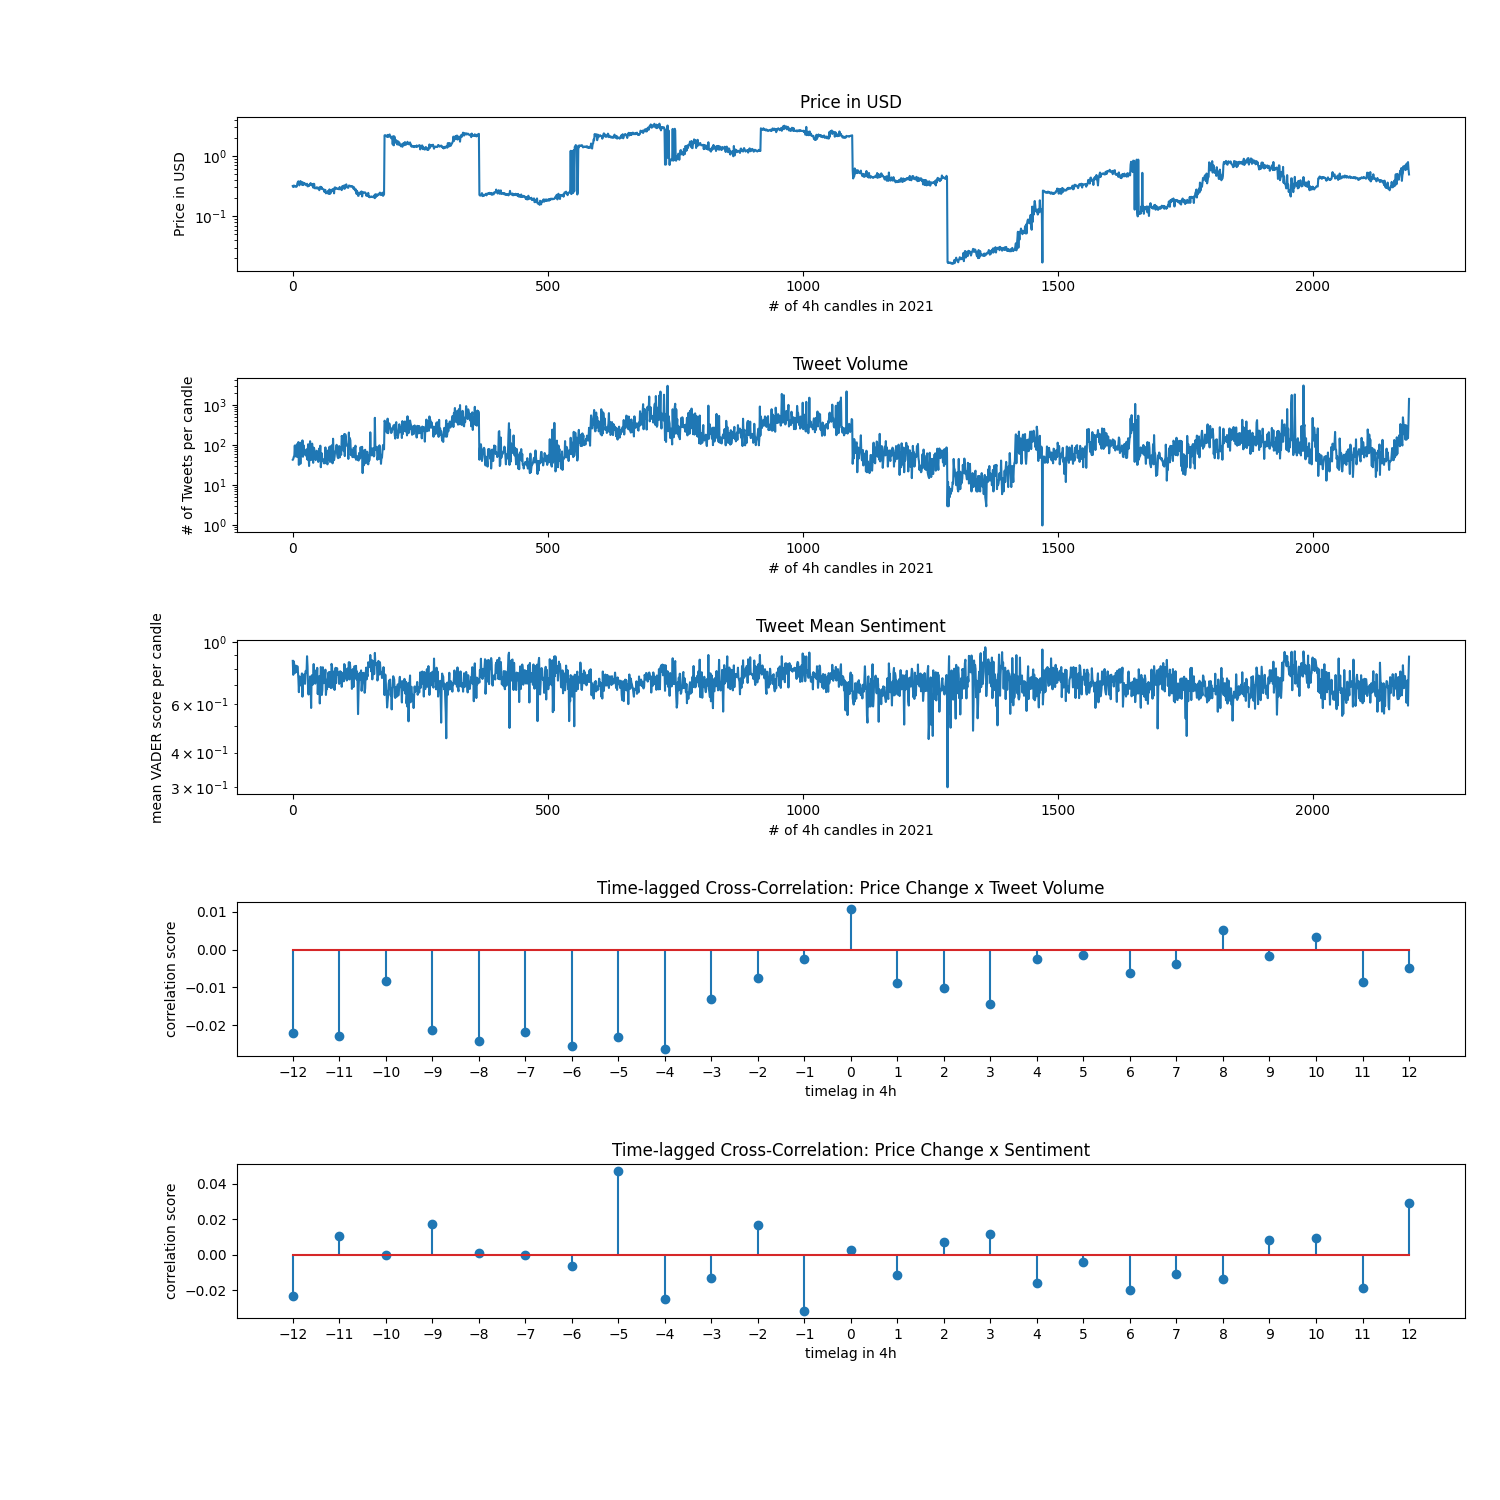
\includegraphics[width=\textwidth]{figures/crosscorrFTM_4h_range(-12, 13).png}
         \caption{FTM 4H}
         \label{ftm4h}
     \end{subfigure}
      \hfill 
     \begin{subfigure}[b]{0.45\textwidth}
         \centering
         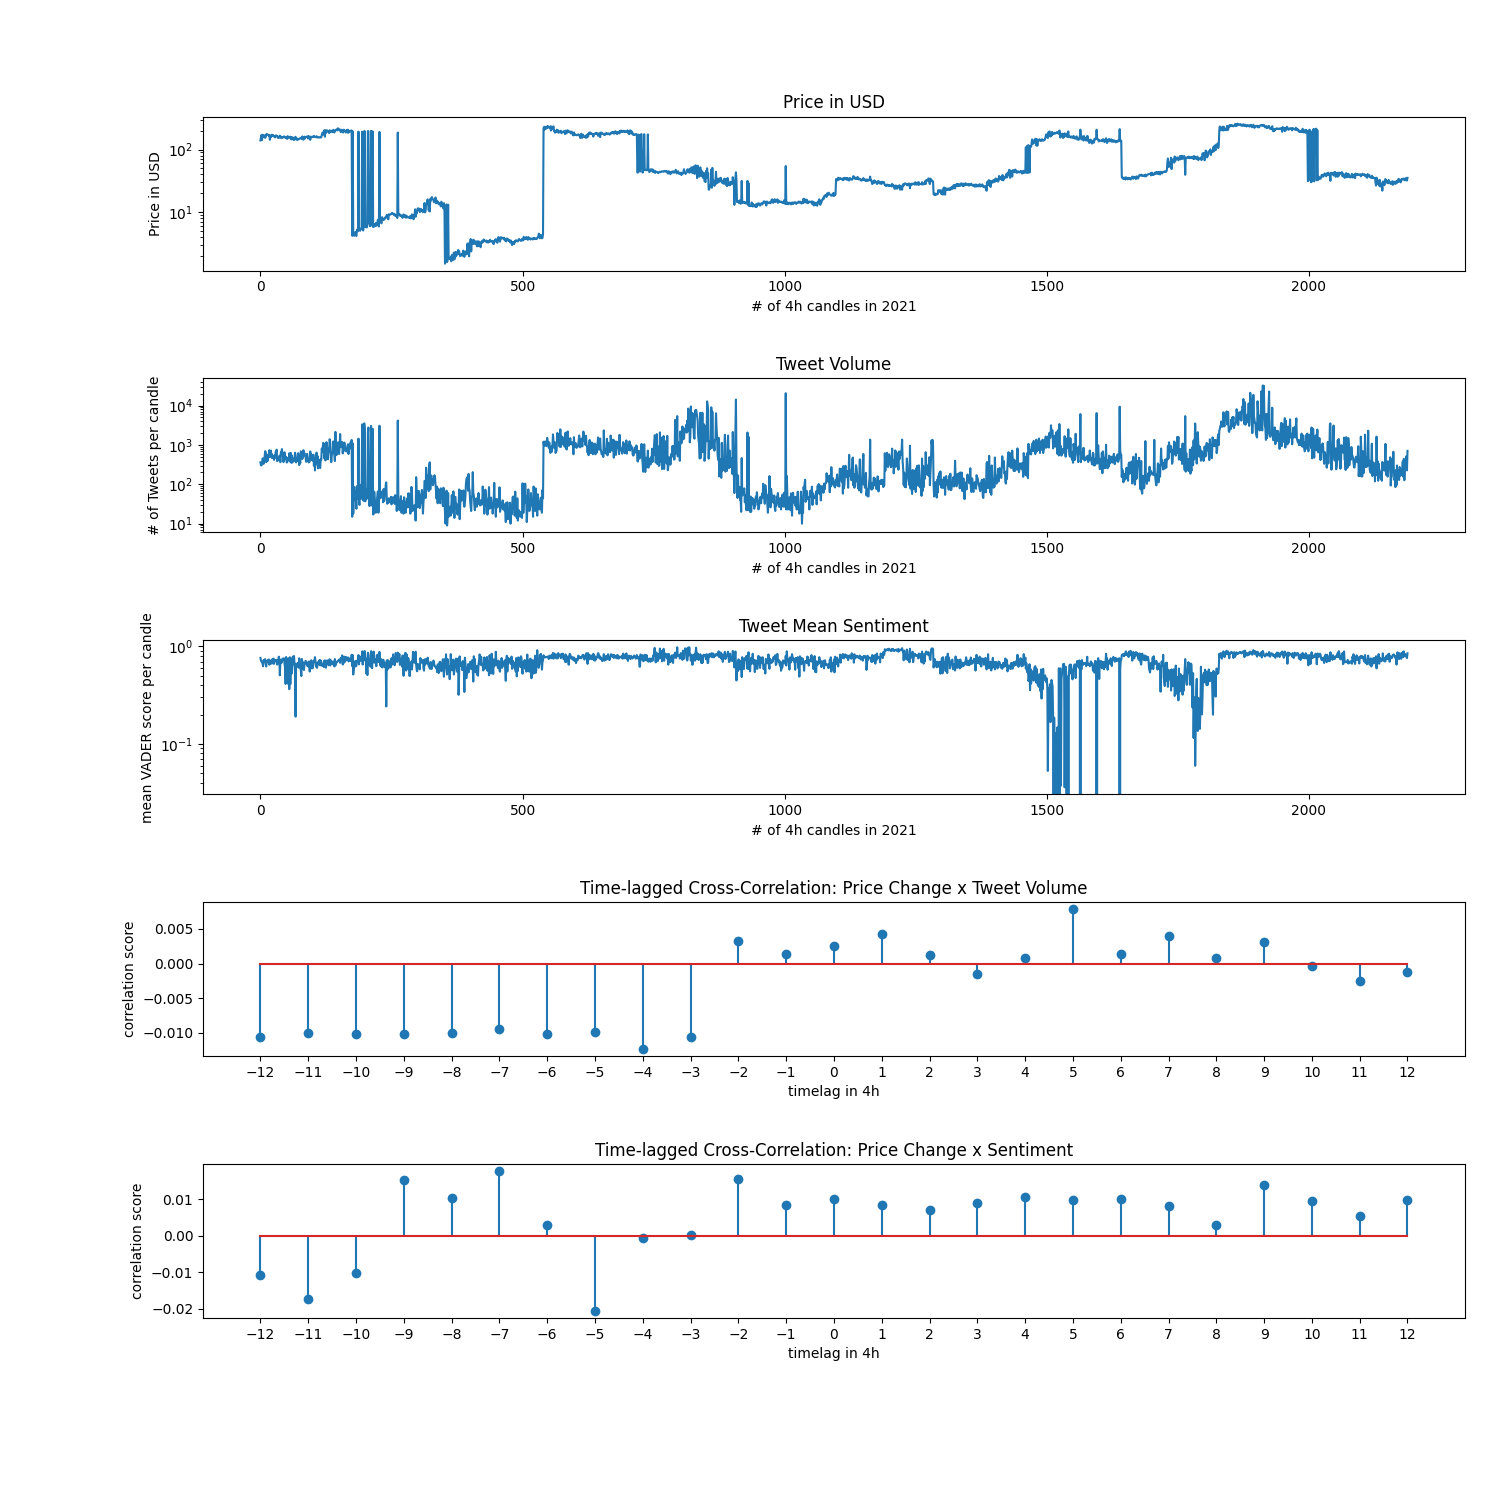
\includegraphics[width=\textwidth]{figures/crosscorrSOL_4h_range(-12, 13).png}
         \caption{SOL 4H}
         \label{sol4h}
     \end{subfigure}
        \caption{Price, Tweet Volume, Tweet Sentiment and Cross-Correlation graphs of Tweet Volume x Price and Tweet Sentiment x Price. This is using the 4h candles for the four chosen Cryptocurrencies.}
        \label{fig:crosscorr-4h}
\end{figure}

\restoregeometry     %so it does not affect the rest of the pages.

Looking at the plotted Cross-Correlation graphs, there are some patterns emerging. Starting with Sentiment, there is a pattern of high correlation on the AVAX 1H data, skewing towards negative time-lag, meaning a correlation of Price Change preceding Sentiment. Using the 4H data, SOL shows a light pattern which implies a correlation when Twitter sentiment precedes Price Change.\\
In general however, much clearer patterns are visible for the Correlation of Price Change and Tweet Volume. The most common pattern is that of a negative correlation when price precedes Volume and a positive when the lag is positive.

\section{Discussion}

\subsection{Interpretation}

The utilised method of transcribing freqency of occurrence of words to VADER scores has improved the classifiers score, despite limited available labelled data. The improved score however, comes with the caveat of an increased bias towards positive classifications, which on the other hand reflect the positive bias in the training data. Thus, the increased performance on the test set, which can be expected to display a similar bias. \\ 
Generally no strong pattern emerges by analyzing sentiment and price correlation. Tweet volume shows a stronger pattern. The aforementioned negative Tweet Volume - Price correlation for negative time-lags can not be interpreted directionally, meaning whether lower price precedes high volume or higher price precedes low volume, one can only speculate about situations, for example one, where a dumping price can trigger many posts on Twitter. \\

\subsection{General Discussion \& Outlook}

Careful thought went into the consideration whether or not to adjust the imbalances of positive, neutral and negative Tweets, as there is a strong bias towards positive sentiment. It could therefore be conceived to, for example in the labelled gold standard set from which the VADER scores are ultimately derived, balance it out to three evenly sized categories. This was not done and as a result, the positive bias of Tweets as they occur in vivo is transferred to the edited VADER classifier, which, however, shows a better performance because it is evaluated and used on biased data. This naturally occurring bias is also one reason as to the decision to not balance the gold standard data set, another is the viability: Achieving balanced data of portions which are meaningfully large had resulted in an amount of labelling work which would have gone beyond the scope of this project. \\
Another point of possible discussion is the decision to exclude non-organic Twitter content via heuristics like hashtag-spamming or filtering by certain key words. Bot content could also be seen as signaling positive sentiment by proxy, by indicating enough interest in or popularity of the particular Cryptocurrency referenced. But since this project is about the nature of the language used, and bot Tweet analysis would have inevitably led to the inclusion of repetitive phrases and statements and an even larger positive bias into the data set, they were chosen not to consider. \\
Certain qualities of the Twitter data became more obvious during more intensive preoccupation during the labelling task. That is for example, even though sentiment may be expressed in Tweets, it is not often clearly separable what the sentiment pertains to. Of course, and especially due to the nature of the chosen Cryptocurrencies which all serve as Layer 1 Blockchain ecosystems for various other products and protocols, they are not seen exclusively as investment vehicles. It follows that sentiment is also expressed about other qualities like security, speed or general user experience. This, of course can be interpreted as a proxy for price expectation but needs to be recognised as separate from statements, for example, expressing sentiments about possible price appreciation, etc. It also often occurs that a tokens ticker tag is used to drag the attention to something else discussed in the Tweet, or that there are multiple entities in the same Tweet and they are contrasted (\textit{A is good, unlike B ...}). Other times there was favourable sentiment towards a Cryptocurrency by mentioning profits made by shorting (betting the price lowering during a certain period), which leads to an interesting paradox in the scope of this project. Such Tweets were chosen to be excluded from the labelled gold standard data set, since the currently used methods have no way of discriminating or recognising entities etc. It would, however, be interesting to include such methods in future research as one method to refine Sentiment Analysis on the data. \\
On trade-off that was made regarding determining and scoring the Crypto-relevant words and their valency was, that due to the relatively small size of the gold standard set, relevant words were determined in an intermediary step using the whole unlabelled corpus sampled from Crypto Tweets. This decision was due to the assumption that the gold standard set was not of sufficient size to really determine a representative set of words critical for Crypto language. Tweets labelled with "neutral" sentiment, and words which ended up with a more neutral score below a certain threshold were also not used for the editing of the dictionary, the reason being that a higher emphasis should be placed on the words which seemed to offer a higher predictiveness, also due to the assumption that, with a small data set size this is needed for bootstrapping an effective classifier.\\
The method chosen for the adjustment of the VADER lexicon was very different from the subjective rater agreement in the original paper. Objectiveness through data and pure frequency analysis was prioritized in this approach to edit the lexicon. However, some subjective performance was exercised in eliminating some clutter which ended up with high VADER scores, such as "..." and in the binning of the PosNeg scores to VADER scores. Other terms like "project" had also ended up with high scores in the edited lexicon, which wold normally not be ascribed positive sentiment but were left alone due to the assumption of some sort of sentiment predictiveness and to favor the quantitative approach. Examples like this brought to the authors attention the difficulties of choosing the right balance between quantitative and qualitative approach and an appreciation for the necessity of occasional manual feature engineering. \\
The aforementioned positive bias is not fully particular to the Twitter data alone; 2021 was for long periods of time what is usually considered as a "bull market" and the 2021 market data is therefore possibly not optimal for a balanced analysis. It is, however, segmented by shorter-term up and down trends. Since the correlation was always computed for the sequence of the whole year, it would be interesting to see if analysis of up-trend or down-trend only segments somehow influence the final analysis results and also to what extent the mood on social media reflects these trends. This is another idea which future research could occupy itself with but can be considered outside of the scope of this project. \\
In this project there were some explorations on how to achieve an effect (in this case in the editing of the VADER classifier) even in the absence of a large set of labelled data (as opposed to brute force methods, often used in the Computational Linguistics and Machine Learning field). For one, out of necessity and time constraints, but also out of a general interest in such approaches. Further research could be focused on a solving this problem even better with a more refined or technical approach than the admittedly simple rule-based mechanism underlying VADER. This approach could take into account semantic information, Parts of Speech, use Pre-Trained Neural Networks, unsupervised methods etc. \\
Generally this project was admittedly on the explorative side due to the broader scope, taking multiple steps which build upon another. This did not always leave enough time for extreme thoroughness or scrutiny to test and optimize parameters against each other. Nonetheless it has led to many interesting conclusions and experiences for the author and will possibly lead to a more constrained approach to some of the aspects dealt with in this research in the near future. \\



% %%%%%%%%%%%%%%%%%%%%%%%%%%%%%%%%%%%%%%%%%%%%%%%%%%%%%%%%%%
% %%%%%%%%%%%%%%%%%%%%%%%%%%%%%%%%%%%%%%%%%%%%%%%%%%%%%%%%%%
% REFERENCES SECTION
% %%%%%%%%%%%%%%%%%%%%%%%%%%%%%%%%%%%%%%%%%%%%%%%%%%%%%%%%%%
% %%%%%%%%%%%%%%%%%%%%%%%%%%%%%%%%%%%%%%%%%%%%%%%%%%%%%%%%%%
\medskip

\bibliography{references.bib} 


% ==========================
% ==========================
% ==========================


\end{document}